\documentclass[a4paper,12pt,oneside,openright]{book}

\usepackage[utf8x]{inputenc}
\PrerenderUnicode{ăîșțâĂÎÂȘȚ„”}
 
\usepackage{bookman}
\usepackage{graphicx}
\usepackage{listings}
\usepackage{fancyhdr} 
\usepackage{color}
\usepackage[T1]{fontenc}
\usepackage{float}
\usepackage{ifthen}
\usepackage{geometry}
\usepackage{indentfirst}
\usepackage{mathptmx}
\usepackage[hyphens]{url}
\usepackage{hyperref}
\usepackage{textcomp}
\usepackage{wrapfig}
\usepackage[romanian]{babel}
\graphicspath{ {./fig/} }

\pagestyle{fancy}
\fancyhead[RE]{\footnotesize{\leftmark}}
\fancyhead[RO]{\footnotesize{\thepage}}
\fancyhead[LO]{\footnotesize{\rightmark}}
\fancyhead[LE]{\footnotesize{\thepage}}
\fancyfoot{}

\renewcommand{\chaptername}{Capitolul}
\renewcommand{\figurename}{Figura}
\renewcommand{\tablename}{Tabelul}
\renewcommand\listtablename{Lista tabelelor}
\renewcommand\listfigurename{Lista figurilor}
\renewcommand\contentsname{Cuprins}
\renewcommand\bibname{Bibliografie}
 
\begin{document}

\newgeometry{centering}
\begin{titlepage}
    \begin{center}
        \begin{minipage}{0.3\textwidth}
                \scalebox{0.25}{
\includegraphics{fig/ACLogo.jpg}}
                \scalebox{0.25}{
\includegraphics{fig/DCTILogo.png}}
        \end{minipage}%
        \begin{minipage}{0.4\textwidth}
            \centering
            \scriptsize
            Universitatea Politehnica Timișoara\\
            Facultatea de Automatică și Calculatoare\\
            Departamentul Calculatoare și \\Tehnologia Informației
        \end{minipage}%
        \begin{minipage}{0.3\textwidth}
            \begin{flushright}
                \scalebox{0.25}{
\includegraphics{fig/UPTLogo.jpg}}
            \end{flushright}
        \end{minipage}
    \end{center}
    
    \noindent\rule{\textwidth}{1pt}\\[5cm]
    
    \begin{center}
        {\huge \bfseries \textsc{Termostat inteligent, controlat printr-o aplicație web}}\\[2cm]
        {\large \bfseries Proiect de Diplomă}\\[2cm]
        \begin{flushright}
            \large
            Autor:\\
	      Vitomir Dragan\\[1cm]
        \end{flushright}
        \begin{flushleft}
            \large
            Conducător științific\\
            Prof. Dr. Habil. Ing. Marius Marcu\\[2cm]
        \end{flushleft}
        {\small Timișoara \\Iunie, 2021}
    \end{center}
\end{titlepage}
\restoregeometry
\shipout\null

\setcounter{page}{1}
\tableofcontents
\chapter{Introducere}\label{ch:1intro}

\section{Internet of things}
	Nivelul de evoluție la care a ajuns tehnologia în zilele noastre, dă naștere dorinței de a spori confortul vieții cotidiene prin creșterea gradului de interconectare al dispozitivelor inteligente.

	Scopul primordial al conceptului de Internet Of Things este de a face posibilă comunicarea între obiectele care prezintă utilitate în viața de zi cu zi. Acesta reprezintă o rețea vastă de dispozitive interconectate care sunt capabile să ia decizii fără intervenție din exterior. Prin intermediul senzorilor sunt preluate diverse date din mediul înconjurător, date care, în urma prelucrărilor, determină execuția anumitor acțiuni.

	Contrar așteptărilor, ideea de Internet of Things nu a apărut recent. Primul dispozitiv care implementa conceptul de IoT a fost lansat în anul 1982, fiind reprezentat de un tonomat de Coca-Cola care putea să trimită informații pe internet referitoare la numărul de doze disponibile si temperatura băuturilor \cite{cokeMachine}. În anul 1990, invenția lui John Romkey, toaster-ul controlat prin internet \cite{simoniot}, stârnește tot mai mult interesul asupra ideii de control de la distanță al dispozitivelor. În decursul anilor, tot mai multe firme producătoare de electronice au încercat să ofere clienților produse care pot transfera date prin intermediul internetutlui. De exemplu, în anii 2000, firma LG a produs un frigider care se putea conecta la internet prin WiFi \cite{simoniot}.

	Chiar dacă dispozitivele care au marcat debutul IoT nu oferă funcționalități mult prea utile, în ultimii ani s-a dovedit că transferul de date între dispozitive, fără a utiliza conductori electrici, poate fi folositor chiar și în domenii cheie. Astfel, medicina, armata, transporturile și imobiliarele sunt doar câteva exemple de domenii care au fost influențate de acest concept.  

	Medicina - se urmărește implementarea conceptului de monitorizare de la distanță, prin intermediul unor aparate care au rolul de a înregistra date legate de starea de sănătate a pacientului și de a le trimite într-o bază de date accesibilă de către personalul medical \cite{medical}.

	Armata - prezintă dispozitive de spionaj și de supreveghere de ultimă generație, toate acestea fiind posibile datorită ideii de Internet of Things \cite{army}.

	Industria transporturilor - în acest domeniu, IoT poate fi ilustrat prin transferul de date între un autovehicul și infrastructură, pietoni sau un alt autovehicul. Acest concept poarta denumirea de V2X, iar beneficiul major pe care îl poate aduce este reducerea considerabilă a numărului de accidente \cite{V2X}.   

	Imobiliare - în zilele noastre, se întâlnește din ce în ce mai des ideea de casă inteligentă. Aceasta se rezumă la faptul că, dispozitivele inteligente din casă comunică atât între ele cât și cu electrocasnicele, reușind sa creeze un mediu cât mai confortabil pentru locuitori.

	Faptul că domeniul IoT prezintă o utilitate care nu poate fi neglijată, explică creșterea exponențială a numărului de dispozitive interconectate. Conform unei statistici publicate de către Arne Holst, conducătorul echipei de cercetare din cadrul companiei Statista, se aproximează ca în 2030 să se ajungă la un număr mai mare de 25.4 miliarde de dispozitive IoT \cite{increaseOfIot}.

\bigskip

\begin{figure}[H]
   	\centering
    	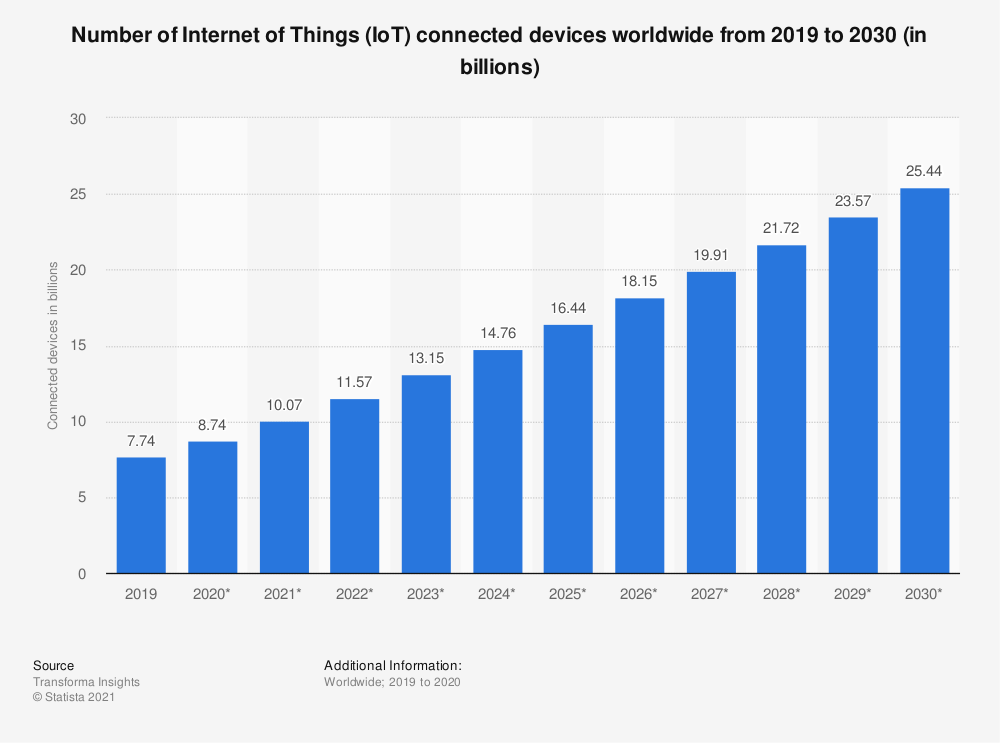
\includegraphics[width=0.8\textwidth]{Statistica-IoT.png}
	\caption{Evoluția numărului de dispozitive IoT (sursa: \cite{increaseOfIot})}
\end{figure}

\section{Contextul de realizare}\label{sec:context}
	Doresc ca prin intermediul proiectului să prezint beneficiile pe care automatizarea și conceptul de IoT le pot aduce. Sistemul creat abordează una dintre problemele care pot interveni la nivelul unei locuințe și se folosește de transferul de date la distanță, între diverse componente electronice, pentru a soluționa disconfortul termic.

	Problema pe care încerc să o rezolv, prin intermediul proiectului, am sesizat-o la apartamentul în care locuiesc. Acesta prezintă două camere de dimensiuni diferite, iar în sezonul rece ne confruntam cu un disconfort termic cauzat de diferențele de temperatură între cele două camere. Termostatul este montat în camera mare, fapt ce determina ca temperatura din camera mică sa fie mai mare decât cea setată. Nici mutarea termostatului in camera mică nu reprezenta o soluție, din cauză că timpul necesar încălzirii camerei mari este mai mare decât cel pentru camera mică, ajungându-se ca în camera mare sa fie tot timpul mai rece. Prin urmare, această inconveniență m-a motivat să creez un sistem care să reușească să mențină o temperatură constantă în apartament.

	La nivel non-tehnic, soluția constă în montarea în fiecare cameră a unor module ce monitorizează temperatura, iar în funcție de aceasta, comandă atât electrovalvele montate pe returul caloriferelor, cât și centrala. Rolul electrovalvei este de a închide sau deschide circuitul de apă din calorifer. De asemenea, este necesar ca lângă centrala termică să se monteze un modul care are rolul de a porni sau de a opri centrala în funcție de comanda primită de la modulele montate în camere. Acest modul se conectează la centrală prin intermediul unor fire, iar transferul de date între modulele din camere și modulul de control al centralei se face prin radio - frecvență. Pot fi setate temperaturi diferite pentru fiecare cameră în parte. Setarea se poate face fizic, prin intermediul unor butoane, sau de la distanță, prin intermediul unei aplicații web sau prin comenzi vocale interpretate de Google Assistant. Sistemul prezintă două moduri de funcționare. Primul mod constă în menținerea temperaturii setate, fără a ține cont de oră sau de faptul că ziua curentă este lucrătoare sau nu. Cel de-al doilea mod, oferă posibilitatea utilizatorului de a seta, prin intermediul aplicației web, temperaturi diferite pe anumite intervale orare ale zilei. Sistemul permite setarea a patru intervale orare în timpul zilelor lucrătoare ale săptămânii, iar pentru weekend pot fi setate două intervale.

\chapter{Prezentarea sistemelor similare}\label{ch:2sistemeSimilare}

	In momentul de față, acest subdomeniu se află la un nivel mare de răspândire. Există o serie de producători care comercializează sisteme ce permit controlul la distanță al temperaturii, însă au o deficență majoră, și anume, prețul ridicat. Voi prezenta mai multe astfel de sisteme, împreună cu detaliile tehnice ale acestora. 	

\section{Torelectric}
	Termostatul produs de firma Torelectric oferă mai multe modalități de reglare a temperaturii:
	\begin{itemize}
  	\setlength{\itemindent}{2em}
		\item Prin aplicație mobilă
		\item Fizic, utilizând interfața termostatului
		\item Prin comenzi vocale, utilizând Google Home și Alexa
	\end{itemize}
	

	\begin{figure}[H]
    		\centering
    	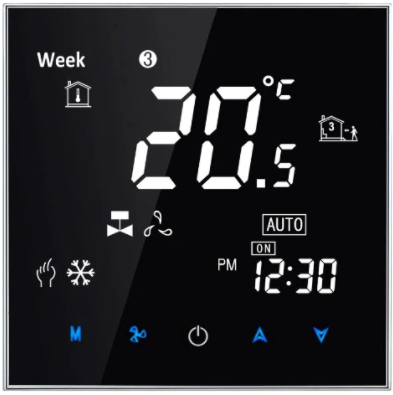
\includegraphics[width=0.4\textwidth]{Torelectric.png}
	\end{figure}

	Ca și caracteristici principale se pot remarca:
	\begin{itemize}
	\setlength{\itemindent}{2em}
		\item Conectivitate: Wi-Fi
		\item Tip alimentare: La retea
		\item Precizie: $\pm 2$ \textdegree{}C sau $\pm 1$ \textdegree{}C
		\item Setare temperatură intre: 5 - 35 \textdegree{}C
		\item Temperatură ambientală: 0 - 45 \textdegree{}C
	\end{itemize}

\begin{wrapfigure}{l}{0.4\textwidth} 
\centering
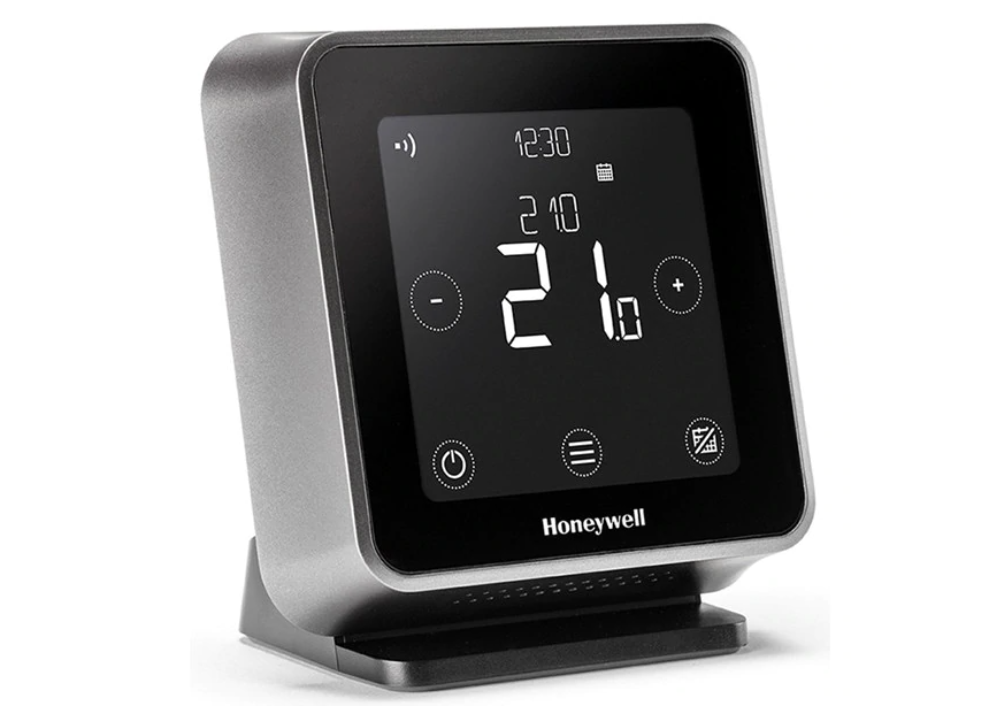
\includegraphics[width=0.4\textwidth]{Honeywell.png}
\end{wrapfigure}
\section{Honeywell}
	Termostatul produs de Honeywell se diferențiază față de cel produs de Torelectric prin prezența unor funcționalități inovatoare. Printre particularitățile acestui dispozitiv se remarcă:
	\begin{itemize}
	\setlength{\itemindent}{2em}
		\item Adaptarea temperaturii în funcție de prezența sau absența unor persoane în locuință 
		\item Programarea temperaturilor pentru șapte zile
		\item Controlul de la distanță, oferit de aplicația mobilă
		\item Setarea temperaturii prin comenzi vocale
	\end{itemize}

	Comparativ cu primul sistem prezentat, cel de la Honeywell se deosebește prin tehnologia Geofencing. Acesta știe când imobilul nu este locuit, iar ca urmare, va dezactiva încălzirea. De asemenea, este capabil să detecteze momentul în care locuitorii sunt în apropierea casei, reușind să încălzească până la temperatura setată.
	Un alt avantaj adus de cei de la Honeywell este posibilitatea de a seta temperatura pe decursul a șapte zile, fapt ce asigură un confort sporit, prin adaptarea temperaturii în funcție de diverse intervale orare.

	Caracteristicile tehnice ale acestuia sunt:
	\begin{itemize}
	\setlength{\itemindent}{2em}
		\item Destinat: centrale termice
		\item Suprafata de montare: masă
		\item Tip alimentare: la rețea
		\item Conectivitate: Wi-Fi
	\end{itemize}

	În continuare, voi prezenta două sisteme care reprezintă apogeul evoluției în acest domeniu. Acestea sunt produse de firme cunoscute precum: Google si Ecobee.

\section{Nest}
	Este un termostat inteligent produs de cei de la Google. Acesta oferă funcționalități avansate pentru un management, cât mai eficient, al temperaturii din imobil. 

	Spre deosebire de sistemele prezentate anterior, termostatele produse de Google Nest integrează tehnologii revoluționare pentru a obține un randament cat mai mare.

\vspace{2em}

	Principalele particularități ale acestuia sunt:
	\begin{itemize}
	\setlength{\itemindent}{2em}
		\item Capacitatea de a se programa automat, în funcție de rutina locuitorilor
		\item Menține temperatura setată doar dacă există persoane în imobil, altfel trece automat la o temperatură ce asigură un consum cât mai mic de energie
		\item Control de la distanță de pe laptop, tabletă și telefon
		\item Salvarea unui istoric al consumului de energie
	\end{itemize}

\vspace{2em}

\begin{wrapfigure}{l}{0.3\textwidth} 
\centering
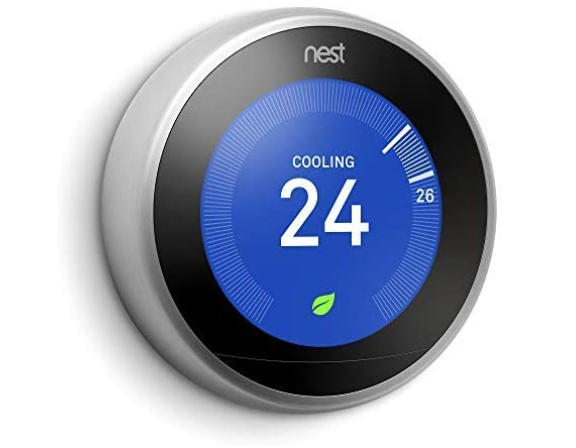
\includegraphics[width=0.3\textwidth]{Nest.png}
\end{wrapfigure}

	Date tehnice:
	\begin{itemize}
	\setlength{\itemindent}{2em}
		\item Sursă de energie: baterii
		\item Tensiune de funcționare: 24 volți
		\item Afișaj digital
		\item Conectivitate: WiFi
	\end{itemize}

\section{Ecobee}
	 Termostatul produs de firma Ecobee poate fi controlat prin intermediul unor aplicații precum: Apple HomeKit, Alexa built-in, Google Assistant, SmartThings. De asemenea, oferă posibilitatea de a seta temperatura de pe Android, dar si de pe iOS.
	
	Acesta implementează un algoritm ce permite controlul temperaturii in diverse locuri din imobil. Se pot conecta mai mulți senzori de temperatura la termostat, iar in funcție de informatiile primite de la aceștia, menține o temperatură constantă în locuință.

	Ecranul se aprinde atunci când detectează o persoană în apropiere, iar pe lângă informațiile legate de temperatură si umiditate, se afișează si vreme pe decursul a cinci zile.

\vspace{2em}

	Date tehnice:
	\begin{itemize}
	\setlength{\itemindent}{2em}
		\item Sursă de energie: baterii
		\item Tensiune de funcționare: 24 volți
		\item Ecran tactil
		\item Conectivitate: WiFi
	\end{itemize}

 
\chapter{Fundamente teoretice}\label{ch:3fundamenteTeoretice}

	În acest capitol voi prezenta principalele concepte teoretice utilizate în realizarea proiectului, împreună cu mediile de dezvoltare, limbajele de programare și framework-urile folosite. 

\section{Medii de dezvoltare}

\subsection{Arduino IDE}

	Pentru programarea plăcuțelor Arduino, se folosește un mediu de dezvoltare numit Arduino Integrated Development Environment. Acesta suportă limbajele de programare C si C++ \cite{arduinoIDE}. 

	Poate rula pe mai multe platforme precum: Windows, Linux, MAC și Java \cite{arduinoIDE}. De asemenea, este important de menționat faptul că este compatibil cu o serie largă de modele de plăcuțe, câteva exemple fiind \cite{arduinoIDE}:
		\begin{itemize}
			\setlength{\itemindent}{2em}
			\itemsep0em
			\item Arduino Uno
			\item Arduino Mega
			\item Arduino Leonardo
			\item Arduino Micro
		\end{itemize} 

	Arduino IDE îndeplinește atât rolul de editor de text, cât și rolul de compilator. Editorul de text reprezintă un suport pentru redactarea codului, iar compilatorul este responsabil de transformarea codului sursă în cod obiect și încărcarea acestuia pe microcontroler \cite{arduinoIDE}.

\subsection{PyCharm}

	Acesta este un mediu de dezvoltare dedicat limbajului de programare \textit{Python}. Prezintă o serie de funcționalități ce facilitează programarea în acest limbaj. Conform \cite{pyCharm}, caracteristicile esențiale oferite de \textit{PyCharm} sunt:
	\begin{itemize}
		\setlength{\itemindent}{2em}
		\itemsep0em
		\item Completare automată de cod.
		\item Refactorizare rapidă și sigură de cod.
		\item Posibilitatea de a crea teste și de a le rula utilizând interfața cu utilizatorul pusă la dispoziție. 
	\end{itemize}
	
\section{Limbaje de programare}

\subsection{Python}

	Python este un limbaj de programare ce a apărut în anul 1991, fiind realizat de către Guido van Rossum \cite{python}. Se bucură de o evoluție fulminantă, ajungând să fie unul din cele mai utilizate limbaje de programare în anul 2020. Creșterea numărului de programatori care aleg să folosească Python este datorată  caracteristicilor precum \cite{python}: 
	\begin{itemize}
	\setlength{\itemindent}{2em}
	\itemsep0em
	\item Flexibilitatea, poate fi utilizat într-un număr vast de domenii, de la programare web, până la programare pe plăcuțe. Funcționează pe o multitudine de platforme, printre care se enumeră: Windows, Mac, Linux și Raspberry Pi. 
	\item În ceea ce privește sintaxa acestui limbaj de programare, este una simplă, care permite scrierea de programe utilizând un număr mai mic de linii de cod. 
	\item Poate fi folosit atât pentru programare procedurală, funcțională, dar și orientată pe obiecte.
	\end{itemize}

\subsection{C++}

	C++ este un limbaj de programare bazat pe C. Motivele pentru care creatorul acestui limbaj de programare, Bjarne Stroustrup, a decis să folosească limbajul C ca punct de plecare sunt: flexibilitatea si faptul că este un limbaj apropiat de partea hardware, rulează pe multe platforme și se potrivește cu mediul de programare UNIX \cite{c++}.

	Ceea ce aduce nou este posibilitatea de a programa orientat pe obiecte, o programare de tip generic și face posibil conceptul de abstractizare al datelor \cite{c++}. Numărul de domenii în care C++ poate fi aplicat crește considerabil datorită introducerii noțunii de programare orientată pe obiecte. Aceasta implică modelarea unor entități din lumea reală, și interacțiunile acestora, prin intermediul claselor. 

\subsection{HTML}

	Acesta este un limbaj de programare utilizat pentru a forma interfața aplicației web din punct de vedere structural. Permite impărțirea paginilor în mai multe secțiuni și crearea unor serii de elemente esențiale utilizate în astfel de aplicații, precum: butoane, tabele, formulare, câmpuri de intrare și multe altele. Mai mult decât atât, oferă și posibilitatea formatării de text.  


\section{Platforme cloud}

\subsection{Heroku}

	Este o platformă cloud ce permite găzduirea aplicațiilor web realizate în diverse limbaje de programare: Ruby, Java, Node.js, Clojure, Scala, Python și PHP \cite{heroku}. După ce aplicația a fost găzduită, aceasta poate fi administrată prin intermediul liniei de comandă pusă la dispoziție de platformă \cite{heroku}.

\subsection{Baza de date în timp real Firebase}

	Este o bază de date găzduită pe cloud, iar informațiile sunt stocate în format JSON \cite{firebase}. De asemenea, nu necesită interogări de tip SQL pentru a stoca sau a citi date și oferă siguranța faptului că datele nu se vor pierde dacă este întreruptă conexiunea \cite{firebase}.

\section{Framework-uri}

\subsection{Flask}

	Este un framework construit pe baza limbajului de programare Python, ce oferă posibilitatea de a dezvolta aplicații web. Faptul că este proiectat ca să fie extins, oferă posibilitatea programatorului de a avea control total asupra aplicației pe care o creează. Prezintă un nucleu robust, care include toate funcționalitățile de bază pe care o aplicație web le necesită, nucleu ce poate fi extins de diverse părți terțe \cite{flask}.

	Pentru a crea aplicații web complexe, utilizarea doar a framework-ului nu este suficientă. Motiv pentru care, flask permite îmbinarea cu limbaje de programare precum javascript, CSS și HTML.

\subsection{Bootstrap}

	Framework utilizat pentru a crea partea de interfață cu utilizatorul, ce combină \textit{HTML}, \textit{CSS} și \textit{JavaScript} \cite{bootstrap}. Prezintă o serie de formulare, meniuri de navigare și multe alte elemente de aspect predefinite.  


\section{Componente utilizate}

\subsection{ESP8266}

	NodeMCU ESP8266 este o placă ce se poate conecta prin WiFi la o rețea de internet. Prezintă o antenă esp8266 ce acceptă standardele 802.11b/g/n și protocolul de securitate WPA/WPA2 \cite{esp8266}. Integrează un modul ADC pe 10 biți, microcontroler pe 32 de biți, ce are un consum redus de energie, și se bazează pe protocolul TCP/IP pentru a face transferul de date \cite{esp8266}.

\subsection{Placă de bază pentru NodeMCU}

	Are rolul de a alimenta modulul wireless ESP8266 și de a oferi o extensie pentru pinii pe care acesta îi pune la dispoziție. In ceea ce privește alimentarea, se face printr-un conector de tip jack și acceptă valori între 6 și 24 de volți. De asemenea, placa de bază integrează un regulator de tensiune ce convertește valoarea tensiunii de intrare la 5 volți.

\subsection{Arduino Uno}

	Arduino aduce pe piață o serie de plăcuțe cu microcontroler, ce pot fi programate pentru diverse aplicații. De asemenea, bibliotecile puse la dispoziție pentru acest tip de sisteme sunt menite să faciliteze procesul de programare al acestora \cite{arduino}.

	Programarea plăcuței se face prin intermediul conectorului USB. Aceasta prezintă și un conector separat pentru alimentare care suportă tensiuni în intervalul 7 - 12 volți \cite{arduino}, tensiuni ce vor trece prin regulatorul de tensiune integrat în plăcuță.

	În ceea ce privește pinii prezenți pe placa Arduino Uno, există 6 intrări analogice \cite{arduino}, 14 terminale care pot fi configurate fie ca intrări, fie ca ieșiri \cite{arduino} și o serie de pini ce furnizează tensiune, 3.3 sau 5 volți.

\subsection{LCD 1602}

	Oferă posibilitatea de a afișa text pe două rânduri, fiecare rând conținând 16 caractere. Transferul de date se face prin protocolul $I^2C$, fapt ce reduce considerabil numărul de pini necesari pentru a conecta LCD-ul la Arduino \cite{lcd}.

\vspace{1em}

	Printre caracteristici se remarcă \cite{lcd}:
 		\begin{itemize}
			\setlength{\itemindent}{2em}
			\itemsep0em
			\item Tensiune de alimentare: 5 volți 
			\item Luminozitatea ecranului se poate regla printr-un potențiometru integrat
		\end{itemize} 
	
\subsection{Senzor DHT11}

	Prezintă două părți componente. Prima componentă are rolul de a citi umiditatea ambientală. Este alcatuită din doi electrozi care se suprapun peste un substrat. În momentul în care umiditatea substratului se modifică, determină o modificare a rezistenței dintre cei doi electrozi, iar microcontrolerul detectează și interpretează această valoare. Componenta termică este formată dintr-un termistor. Pe baza valorii rezistenței date de termistor, se vor face prelucrări ajungându-se la o valoare validă a temperaturii.

\subsection{Modul radio frecvență}

	Pereche formată dintr-un transmițător și receptor. Construite pentru a facilita transferul de date prin radio-frecvență. Acestea funcționează la o frecvență de 433Mhz \cite{rfModule}, iar distanța de transmisie diferă în funcție de tensiunea de alimentare a transmițătorului și de calitatea antenelor.

	Conform \cite{rfModule}, se pot evidenția următoarele caracteristici:
 		\begin{itemize}
			\setlength{\itemindent}{2em}
			\itemsep0em
			\item Distanța de transfer: 20 - 200 metri
			\item Tensiune de alimentare transmițător: 3.5 - 12 volți
			\item Rată de transfer: 4 KB/S
			\item Tensiune de alimentare a receptorului: 5 volți
		\end{itemize} 

\subsection{Releu}

	Funcționează ca un întrerupător într-un circuit electric. Principiul de bază al unui releu constă în alăturarea unui solenoid și a unor contacte metalice. În momentul în care solenoidul este alimentat, acesta produce un câmp electromagnetic ce va acționa contactele metalice, deschizând sau închizând circuitul. Releele pe care le utilizez funcționează la 5 volți și au o structură puțin mai complexă, structură pe care intenționez să o detaliez. Prezintă trei intrări: VCC, GND și IN, unde pinii de VCC si GND sunt alimentați permanent, iar IN este pinul de semnal. Acesta este legat la baza unui tranzistor, iar în funcție de tensiunea pe care o furnizează, tranzistorul trece în regim saturat sau blocat, funcționând ca un întrerupător pentru solenoid. De asemenea, în paralel cu bobina este montată o diodă ce are ca și scop protejarea tranzistorului de șocurile de tensiune ce pot apărea la deconectarea alimentării bobinei. Este necesară utilizarea releului pentru a putea controla, prin semnale de putere mică, dispozitive ce funcționează la tensiuni și curenți mari. 

\subsection{Electrovalvă}

	Este un mecanism ce are ca rol deschiderea circuitului de apă în momentul în care este conectat la o sursă de tensiune. Acesta este format dintr-un solenoid și un obturator. Electrovalvele pe care le folosesc sunt de tip normal închis, ceea ce înseamnă că atunci când solenoidul nu este alimentat, obturatorul stă în poziție închis, iar circuitul de apă prin electrovalvă este blocat. În momentul alimentării solenoidului, câmpul magnetic produs de acesta va acționa obturatorul, făcând posibilă trecerea apei prin electrovalvă.

\subsection{Pompă de apă}

	Este alcătuită dintr-un motor electric ce funcționează la 12 volți, curent continuu și acționează o paletă ce pune în mișcare apa din circuit.   

\subsection{Push buton}

	Este un intrerupător, fără reținere, ce are rolul de a trimite semnale către microcontroler. Prezintă două contacte metalice care închid circuitul în momentul în care se ating. 

\subsection{Condensator}

	Este o componentă electrică pasivă ce are rolul de a înmagazina tensiune. Acesta se utilizează în circuitele electrice pentru a reduce fluctuațiile de tensiune ce pot apărea.

\subsection{Rezistență}

	Asemenea condensatorului, rezistența se încadrează în categoria componentelor electrice pasive. Aceasta are rolul de a se opune trecerii curentului electric. 

\subsection{Circuit integrat Schmitt-Trigger}

	Acesta este utilizat pentru a transforma un semnal analog într-un semnal digital, dar prezintă și rolul de inversor. Dacă se aplică la intrare un semnal cu nivel logic 1, la ieșirea din circuitul integrat va avea nivelul logic 0.

\subsection{Diodă}

	Limitează trecerea curentului electric într-un singur sens, de la anod la catod. Prezintă multe utiliăți în circuitele electrice, un exemplu practic fiind conversia curentului alternativ în curent continuu. 

\section{Filtrarea semnalelor}

	Butoanele pe care le-am folosit, pentru setarea temperaturii dorite, sunt formate din contacte metalice. În momentul în care acestea se ating, produc o vibrație pe care microcontrolerul o percepe ca o apăsare multiplă a butonului. Pentru a rezolva această problemă este necesară crearea unor filtre trece - jos \cite{buttonDebouncing} pentru fiecare buton în parte. Rolul acestor filtre este de a permite trecerea semnalelor cu frecvență mică si de a opri semnalele cu frecvențe mari. Pentru aceasta, am utilizat circuite RC serie, iar valorile rezistenței si condesatorului au fost calculate utilizând ecuația de încărcare și de descărcare a condensatorului. De asemenea, pentru a obține o filtrare cât mai bună, am utilizat un circuit integrat Schmitt-Trigger. Caracteristica datorită căreia acesta îmbunătățește filtrarea semnalului este histereza pe care o are între pragul superior, declanșează trecerea pe nivel logic 0, și pragul inferior, declanșează trecerea pe nivel logic 1.  
\vspace{1em}\\
Conform \cite{buttonDebouncing}, ecuația de încărcare a condensatorului este:

\begin{equation}
V_{cap} = V_{in}(1-e^{\frac{-t}{RC}})
\end{equation}
\vspace{1em}\\
Conform \cite{buttonDebouncing}, ecuația de descărcare a condensatorului este:

\begin{equation}
V_{cap} = V_{in}(e^{\frac{-t}{RC}})                 
\end{equation}
\vspace{1em}\\
$V_{cap}$ - tensiunea stocată în condensator la momentul t
\vspace{0.7em}\\
$V_{in}$ - tensiune de alimentare a circuitului
\vspace{0.7em}\\
t - timpul măsurat din momentul aplicării tensiunii de alimentare la bornele circuitului, în cazul ecuației de încărcare a condensatorului. Pentru ecuația de descărcare a condensatorului, reprezintă timpul măsurat din momentul întreruperii alimentării circuitului
\vspace{0.7em}\\
R - valoarea în ohmi a rezistenței utilizate
\vspace{0.7em}\\
C - valoarea în farazi a condensatorului utilizat\\ 

\vspace{1em}
	În continuare, pentru a putea aplica formulele, este necesară aflarea timpului cât durează oscilația semnalului. Pentru aceasta, am utilizat un osciloscop ce permite analiza semnalului provenit de la buton.

\begin{figure}[H]
	\centering
    	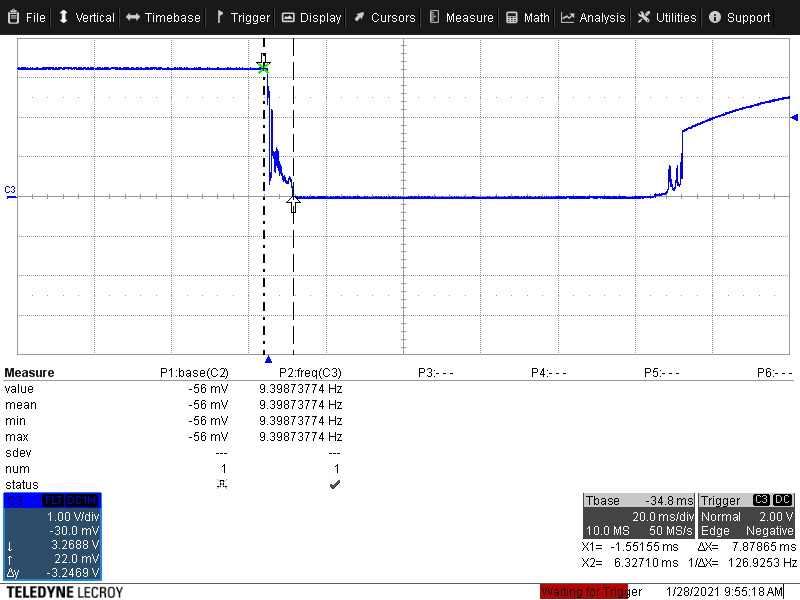
\includegraphics[width=0.8\textwidth]{InainteDeFiltru.jpg}
	\caption{Semnal înainte de filtrul trece jos}
	\label{fig:InainteDeFiltru}
\end{figure}

\begin{figure}[H]
   	\centering
    	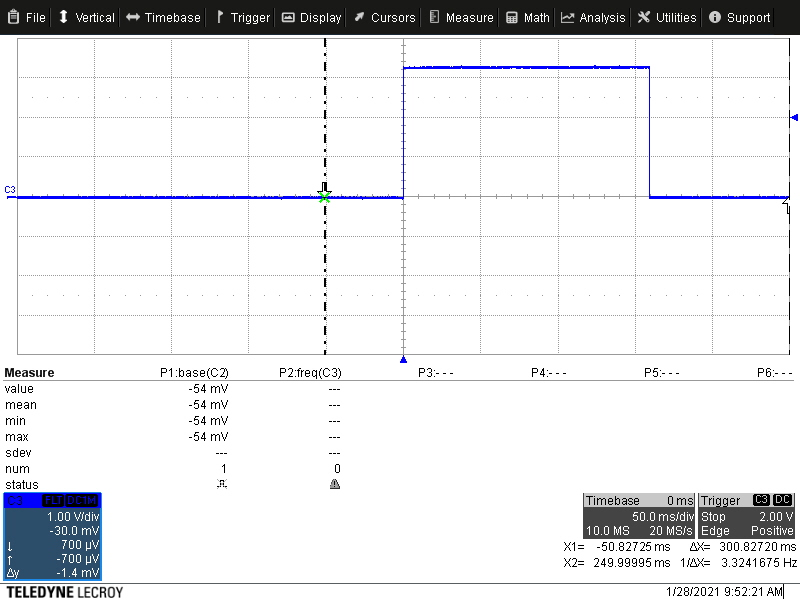
\includegraphics[width=0.8\textwidth]{DupaFiltru.jpg}
	\caption{Semnal după filtrul trece jos}
	\label{fig:DupaFiltru}
\end{figure}
	
	În urma analizei mai multor semnale de la push buton, cea mai mare perturbație a durat aproximativ 8 ms. În calculul valorii rezistențelor si condensatorului care trebuie folosite în filtrele trece - jos, voi folosi un timp de 10 ms. Cele 2 ms în plus reprezintă o marjă de siguranță pentru situațiile în care apar perturbații mai mari decât cele măsurate. 

\vspace{1em}

	În cele ce urmează, voi prezenta schema filtrului trece - jos, iar pe baza acesteia voi detalia calculele realizate pentru a determina valorile componentelor electrice utilizate.

\begin{figure}[H]
   	\centering
    	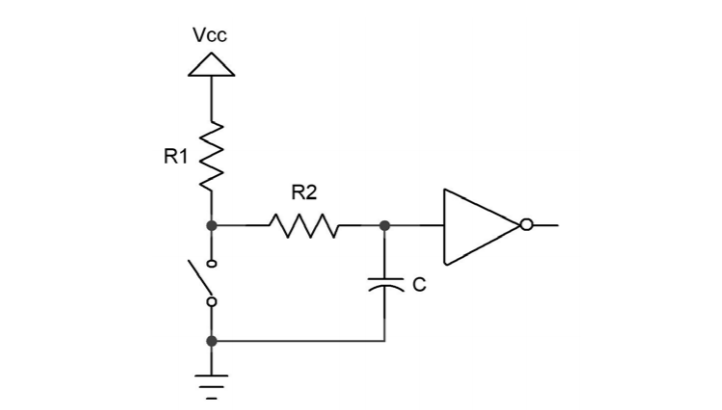
\includegraphics[width=0.6\textwidth]{CircuitRC.png}
	\caption{Schemă filtru trece - jos (sursa: \cite{buttonDebouncing})}
\end{figure}

	În momentul în care întrerupătorul se închide, condensatorul începe să se descarce prin intermediul rezistenței $R_2$. Cunoscând acest aspect, voi putea calcula valoarea $R_2$ utilizând ecuația de descărcare a condensatorului. Valoarea lui t va fi de 10 ms, $V_{in}$ este echivalent cu 3.3 volți(tensiunea la care funcționează modulul WiFi), $V_{cap}$ este egal cu valoarea pragului inferior al inversorului Schmitt-Trigger, iar valoarea condensatorului o aleg de 1 µF. Mai exact, se calculează rezistența astfel încât, după t = 10 ms de la începerea descărcării, tensiunea stocată în condensator să ajungă la valoarea de prag a circuitului integrat.

\[
	R_2 = \frac{-t}{C\ln(\frac{V_{cap}}{V_{in}})} = \frac{-10 \cdot 10^{-3}}{10^{-6}\ln(\frac{1}{3.3})} = \frac{-10}{\ln(0.3)}\cdot 10^3 =  \frac{-10}{-1.2}\cdot 10^3 = 8.33 \cdot 10^3 = 8.33 K\Omega
\]

	Când se deschide întrerupătorul, condensatorul începe să se încarce prin intermediul rezistențelor $R_1$ și $R_2$. Pornind de la această informație, voi calcula valoarea $R_1 + R_2$ utilizând ecuația de încărcare a condensatorului. Doar valoarea parametrului $V_{cap}$ se modifică, va fi echivalentă cu pragul superior al inversorului. 

\[
	R_1 + R_2 = \frac{-t}{C\ln(1 - \frac{V_{cap}}{V_{in}})} = \frac{-10 \cdot 10^{-3}}{10^{-6}\ln(1 - \frac{1.5}{3.3})} = \frac{-10}{\ln(0.54)}\cdot 10^3 =  \frac{-10}{-0.61}\cdot 10^3 = 16.39 \cdot 10^3
\]
\[
	 = 16.39 K\Omega
\]
\[
	R_1 + R_2 = 16.39 K\Omega, R_2 = 8.33 K\Omega \Rightarrow R_1 = 8.06 K\Omega
\]	
	
\section{Histereza}

	Pentru a evita crearea unui lanț de porniri si opriri repetate, pe perioade scurte de timp, cauzate de fluctuațiile rapide de temperatură, este necesară implementarea conceptului de histereză. Acesta constă în stabilirea unei valori de toleranță la temperatura setată, astfel încât diferența de temperatură din momentul în care se trimite comandă pentru oprirea sistemului de încălzire, până la următoarea pornire a acestuia, să fie egală cu dublul valorii histerezei. Cu alte cuvinte, comanda de pornire a încalzirii se va da când temperatura în cameră ajunge să fie mai mică sau egală cu valoare temperaturii setate, din care se sustrage valoarea histerezei. Comanda de oprire va fi declanșată când temperatura ambientală este mai mare sau egală cu valoarea temperaturii setate, la care se adaugă valoare histerezei. În acest fel, timpul între comenzi este mai mare și numărul de cicluri pornit/oprit este mai mic, măsură ce este menită să protejeze sistemele de încălzire.


	 
 
%\chapter{Dezvoltarea soluției}\label{ch:4dezvoltareaSolutiei}

	Acest capitol conține o prezentarea detaliată a modului în care a fost implementat proiectul. Voi face referiri atât la partea hardware, cât și la partea software. 

\section{Specificarea cerințelor}
	
	Redactarea cerințelor sistemului reprezintă o etapă esențială în crearea oricărui proiect. Acestea dictează comportamentul produsului final, fiind necesare atât în faza de dezvoltare, cât și în cea de testare. Cu ajutorul diagramelor cazurilor de utilizare, voi detalia cerințele sistemului descris în această lucrare.

\subsection{Cerințele funcționale ale aplicației web}

\begin{figure}[H]
   	\centering
    	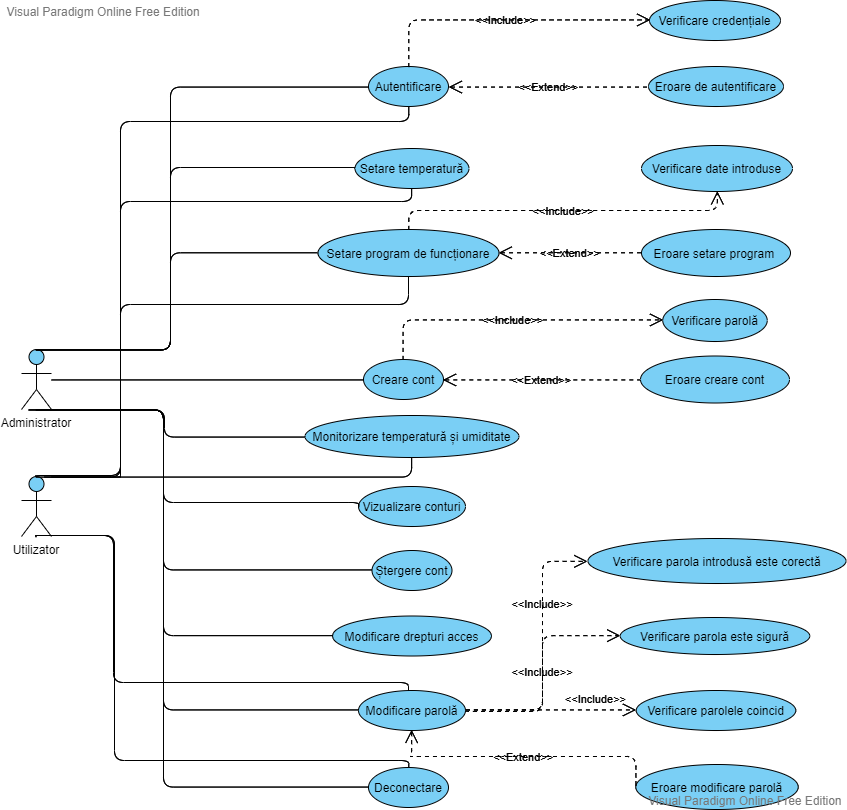
\includegraphics[width=1\textwidth]{Use-Case site.png}
	\caption{Cazurile de utilizare pentru aplicația web}
\end{figure}
	
	Prima cerință pe care aplicația trebuie să o îndeplinească este de a permite utilizatorilor să se autentifice cu ajutorul credențialelor, indiferent de rolul utilizatorului. De asemenea, trebuie tratate situațiile în care parola este greșită sau contul nu există în baza de date.

	Prin intermediul aplicației web, orice utilizator trebuie să poată monitoriza valoarea temperaturii și umidității din imobil.

	Setarea temperaturii trebuie să fie posibilă prin intermediul aplicației web, iar această acțiune nu depinde de rolul utilizatorului.

	O cerință esențială a sistemului este de a oferi posibilitatea setarii, de la distanță, a unui program de funcționare. Această funcționalitate trebuie să fie accesibilă atât pentru conturile cu drepturi de administrator, cât și pentru cele fără. Este necesar ca datele introduse de utilizator să fie verificate și semnalate cazurile în care valorile temperaturilor nu sunt valide sau intervalele nu sunt setate în ordine cronologică.

	Pentru a putea gestiona accesul la aplicație, aceasta trebuie să permită administratorilor să creeze, să șteargă conturi pentru alte persoane și să modifice drepturile de acces ale tuturor conturilor salvate în baza de date. Prin urmare, apare nevoia de noi funcționalități, precum: creare cont, ștergere cont și modificare drepturi de acces. La crearea unui cont, se va verifica dacă parola introdusă este una sigură. Validarea se face pe baza a trei criterii: parola trebuie să conțină cel puțin 6 caractere, cel puțin o literă mare și cel puțin o cifră. În cazul în care nu se respectă condițiile, utilizatorul trebuie să fie avertizat, iar contul nu va fi creat. 

	Cele 3 cerințe menționate mai sus duc la apariția unei noi cerințe. Pentru a facilita stergerea conturilor și modificarea drepturilor de acces, aplicația web trebuie să pună la dispoziție o pagină care să afișeze toate conturile existente în baza de date. Aceasta trebuie să fie accesibilă doar administratorilor.
	 
	De asemenea, din motive de securitate, trebuie ca fiecare utilizator să poată să iși modifice parola. Acest caz de utilizare implică mai multe validări. Este necesar să se verifice dacă parola actuală introdusă este cea corectă. După aceea, identic cazului de utilizare modificare parolă, se verifică dacă noua parolă introdusă este una sigură. În cele din urmă, trebuie verificat dacă parola noua și confirmarea acesteia coincid. Nerespectarea condițiilor duce la afișarea unui mesaj de eroare și la nefinalizarea acțiunii de schimbare a parolei.

	După finalizarea acțiunilor dorite, utilizatorii trebuie să se poată deconecta de la aplicație. 	 

\subsection{Cerințe nefuncționale ale aplicației web}

	În continuare, voi enumera cerințele legate de securitate:
	\begin{itemize}
		\setlength{\itemindent}{2em}
		\itemsep0em
		\item Permisiunile de acces pot fi modificate doar de administratori.
		\item Toate parolele trebuie să fie criptate.
		\item Parolele trebuie să fie complexe. 
	\end{itemize} 

\vspace{1em}

	De asemenea, pe partea de performanță:
	\begin{itemize}
		\setlength{\itemindent}{2em}
		\itemsep0em
		\item Aplicația web trebuie să poată monitoriza parametrii ambientali și seta temperatura într-un imobil cu două camere.
		\item Valorile afișate pe pagina principală trebuie actualizate doar în momentul în care acestea se modifică în baza de date. Nu se acceptă ca actualizările să se execute la anumite intervale de timp prestabilite. 
	\end{itemize} 

\subsection{Cerințe funcționale pentru componentele electronice}

\begin{figure}[H]
   	\centering
    	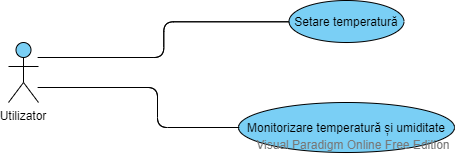
\includegraphics[width=0.8\textwidth]{Use-Case hardware.png}
	\caption{Cazurile de utilizare pentru ansamblul de componente electronice}
\end{figure}	

	Ansamblul componentelor electronice trebuie sa permită modificarea temperaturii setate. Pentru aceasta, se utilizează butoane, iar modificările de temperatură se afișează pe LCD.

 	Pentru a face posibilă monitorizarea parametrilor ambientali, modulele WiFi trebuie să afișeze pe LCD valorile citite de senzorul de temperatură și umiditate. 

	Dacă nu există o conexiune la internet în momentul în care sistemul este pornit, este necesar să se considere valoarea prestabilită de 21 °C ca fiind temperatura ce trebuie menținută în imobil. În cazul întreruperii conexiunii la internet în timpul funcționării, trebuie ca ultima valoare a temperaturii dorite, citită din baza de date, să rămână salvată în sistem.  

\subsection{Cerințe nefuncționale pentru componentele electronice}
	
	O serie de cerințe arhitecturale ale sistemului sunt:
	\begin{itemize}
		\setlength{\itemindent}{2em}
		\itemsep0em
		\item Sistemul trebuie să ruleze într-un regim continuu, zi și noapte.
		\item Pentru a facilita montajul sistemului, trebuie ca transferul comenzilor între modulele senzor și modulul de control să se facă prin radio-frecvență.
		\item Distanța maximă de transfer între modulele senzor și modulul de control trebuie să fie de 200 de metri, în spațiu deschis. 
	\end{itemize} 

\vspace{1em}

	Pe partea de siguranță, este necesar ca:
	\begin{itemize}
		\setlength{\itemindent}{2em}
		\itemsep0em
		\item Centrala termică să fie oprită dacă transferul de date intre modulele senzor și modulul de control este întrerupt mai mult de 5 secunde.
	\end{itemize}
	
\vspace{1em}

	În ceea ce privește fiabilitate:
	\begin{itemize}
		\setlength{\itemindent}{2em}
		\itemsep0em
		\item Sistemul trebuie să poată funcționa și în cazul întreruperii conexiunii la internet.
		\item Pentru a evita situațiile în care o comandă nu este recepționată, transferul datelor între modulele senzor și modulul de control trebuie să se facă ciclic.
	\end{itemize}
 

\section{Arhitectura sistemului}

\begin{figure}[H]
   	\centering
    	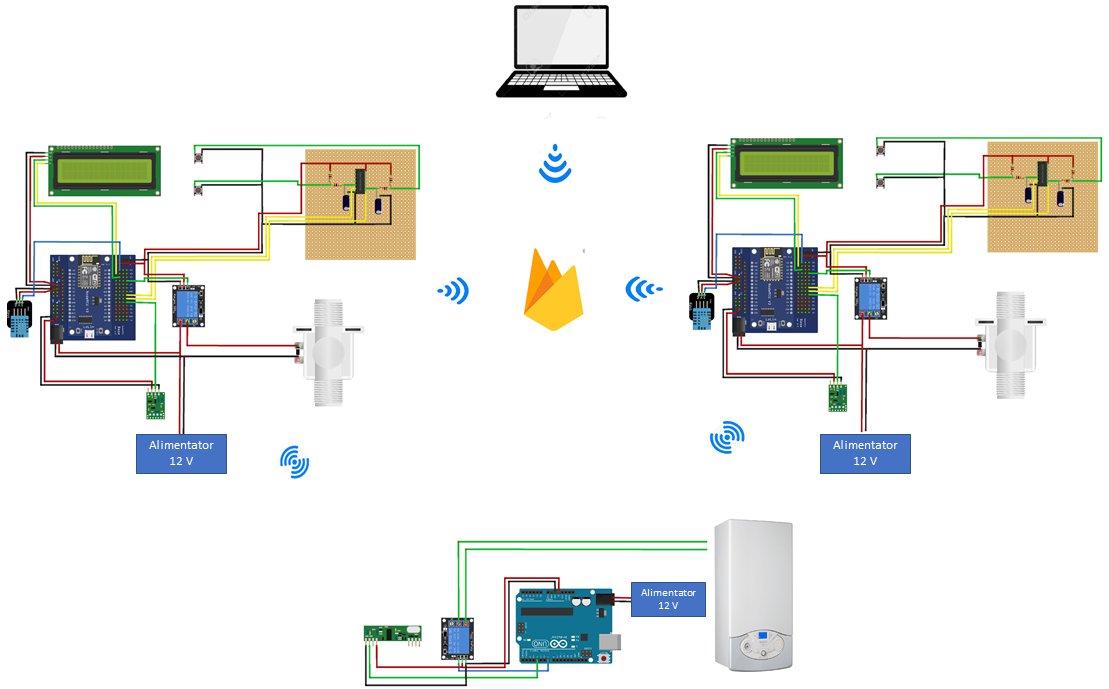
\includegraphics[width=1\textwidth]{ArhitecturaSistemului.png}
	\caption{Arhitectura sistemului}
\end{figure}

	Sistemul a fost conceput pentru un apartament cu două camere, însă poate fi extins pentru un număr mai mare de încăperi. La nivel macro, este format din trei module, câte un modul senzor pentru fiecare cameră și un modul de control, montat în apropierea centralei termice.

	Modulul senzor prezintă o complexitate mai mare, este alcătuit din mai multe componente și îndeplinește o serie de funcționalități. Preia informații precum: temperatura și umiditatea și le trimite în baza de date. În continuare, aceste valori sunt afișate utilizând aplicația web, făcând posibilă monitorizarea parametrilor ambientali. De asemenea, are acces la temperatura setată, iar in funcție de aceasta, dar și de temperatura curentă din cameră, controlează electrovalva și trimite comandă de oprire sau pornire a centralei. Un alt rol esențial pe care îl îndeplinește modulul este de a face posibilă setarea unei valori a temperaturii ce urmează să fie menținută în cameră.

	Modulul de control este de o complexitate redusă. Primește comenzi de la modulele senzor, le interpretează, iar pe baza acestora controlează centrala. Modulul se folosește de logică de tip "SAU", dacă cel puțin un modul senzor trimite comandă de pornire, atunci centrala termică trebuie să înceapă ciclul de încălzire.

	Transferul de date între modulele senzor și modulul de control se face prin intermediul undelor radio, 433 MHz. Placuțele ESP8266 se folosesc de unde Wi-Fi, 2.4 GHz, pentru a se conecta la router.

\subsection{Modulul senzor}

\begin{figure}[H]
   	\centering
    	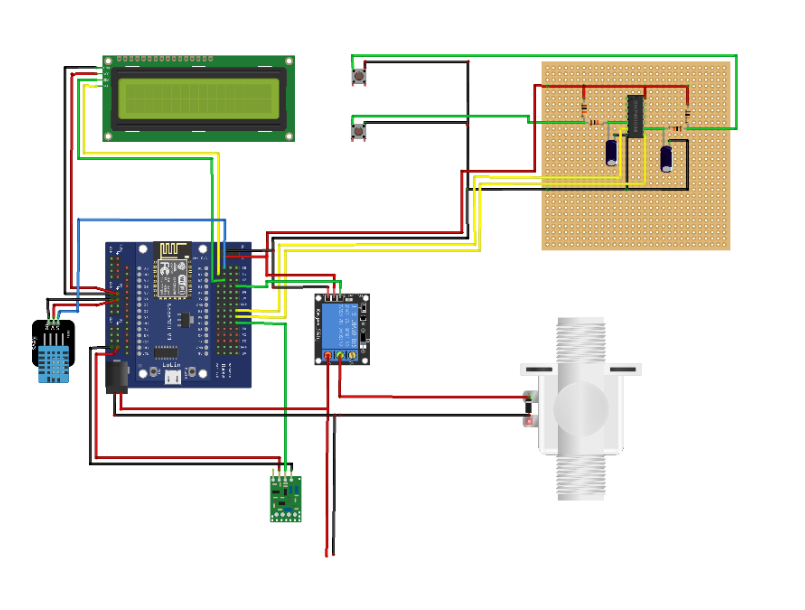
\includegraphics[width=1\textwidth]{ModulSenzor.png}
	\caption{Arhitectura modulului senzor}
\end{figure}	

	Este format din următoarele componente:
	\begin{itemize}
		\setlength{\itemindent}{2em}
			\itemsep0em
			\item Modul WiFi NodeMCU
			\item Placă de bază pentru NodeMCU
			\item LCD
			\item Senzor de temperatură și umiditate
			\item Releu
			\item Butoane
			\item Transmițător RF
			\item Electrovalvă
			\item Circuit integrat Schmitt-Trigger
			\item Rezistență
			\item Condensator
			\item Alimentator 12 volți
	\end{itemize}

	Componenta principală din acest ansamblu este modulul wireless. Se conectează prin WiFi la un punct de acces al rețelei, router-ul în cazul proiectului prezentat, și face transfer de date cu baza de date utilizată. Acesta pune la dispoziție o serie de pini pentru a putea conecta diverse componente auxiliare. 
	
	Pinul D0 este utilizat pentru a conecta pinul de date de la senzorul de temperatură și umiditate.

	Pinii D1 și D2 se conectează la pinii SCL și SDA pentru a face posibil transferul de date prin protocolul de comunicație $I^2C$.

	Pinul D3 se conectează la pinul IN al releului și are rolul de a controla închiderea sau deschiderea releului, iar pinii D5 și D6 sunt rezervați pentru butoane. 

	Pinul D7 transferă date la pinul de date al transmițătorului RF. 

\vspace{1em}

	Placa de bază pentru modulul WiFi are două roluri esențiale în crearea circuitului. Acesta facilitează felul în care se poate alimenta plăcuța wireless, punând la dispoziție un conector de alimentare care este compatibil cu alimentatoare ce furnizează tensiuni între 6 și 24 de volți. Prin intermediul unui regulator de tensiune, va aduce tensiunea de alimentare a modulului WiFi până la 5 volți, prevenind orice posibilitate de supraalimentare. Astfel, placa de bază pune la dispoziție pini ce oferă tensiuni de ieșire de 3.3 volti, 5 volți și o serie de pini ce sunt conectați direct la conectorul de alimentare și furnizează voltaj egal cu cel dat de alimentator. De asemenea, oferă pentru fiecare pin al modulului ESP8266 încă 4 pini corespondenți, fapt ce reprezintă un avantaj când vine vorba de conectarea unor componente auxiliare.

\vspace{1em}

	Pentru a putea afișa temperatura curentă din cameră și temperatura setată, se folosește un display. Transferul de date între LCD și modulul WiFi, la care este conectat, se face prin intermediul protocolului de comunicație $I^2C$. S-a ales acest protocol deoarece reduce considerabil numărul de fire necesare pentru conectarea și alimentarea LCD-ului, în acest caz fiind necesare doar 4. Prin urmare, display-ul pune la dispoziție următorii pini:  VCC, GND, SDA și SCL.

\vspace{1em}

	Senzorul de temperatură și umiditate pe care îl utilizez prezintă 3 pini. Doi sunt utilizati pentru alimentare, VCC și GND, iar cel de-al treilea este pinul de date, utilizat pentru transferul de informații între senzor și plăcuța cu microcontroler la care este conectat.

\vspace{1em}

	Releul este conectat la modulul wireless și este controlat de acesta prin pinul IN. Rolul releului este de întrerupător în circuitul electric format din electrovalvă și alimentator.

\vspace{1em}

	Sunt prezente două butoane ce permit modificarea temperaturii setate. Butonul de sus incrementează temperatura și se conectează la pinul D5 al modului WiFi, iar butonul de jos decrementează valoarea temperaturii și se conectează la pinul D6.

\vspace{1em}

	Transmițătorul RF prezintă 3 pini: VCC, GND și DATA. Pinii VCC și GND se conectează la o sursă de tensiune, ieșirile de 12 volți oferite de placa de bază NodeMCU. Pinul de date se conectează la pinul digital D7 al modulului wireless și face posibil transferul de date între acestea. În continuare, datele vor fi transferate la receptorul de tip RF, montat pe modulul de control.  

\vspace{1em}

	Electrovlava se montează pe returul caloriferelor și este responsabilă de închiderea sau deschiderea circuitului de apă din calorifer. Releul este cel care întrerupe, sau nu, alimentarea electrică a electrovalvei.

\vspace{1em}

	Circuitul integrat Schmitt-Trigger, rezistența și condensatorul sunt componente electrice pe care le-am utilizat pentru a filtra semnalul provenit de la buton.  

\subsection{Modulul de control}

\begin{figure}[H]
   	\centering
    	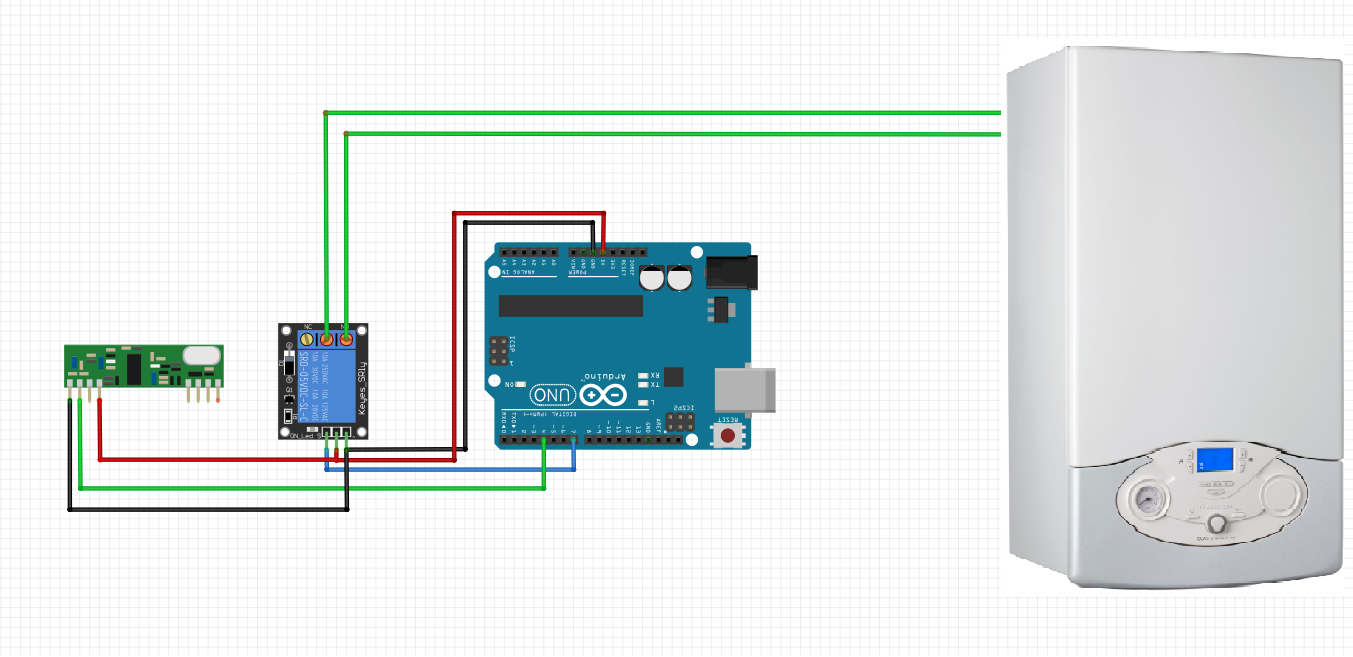
\includegraphics[width=1\textwidth]{ModululDeControl.png}
	\caption{Arhitectura modulului de control}
\end{figure}

	Acesta nu prezintă conexiune la internet. Modulul wireless este înlocuit cu o plăcuță Arduino Uno, care se ocupă de partea de procesare a datelor primite de la modulele din camere. Prezintă o serie de intrări și ieșiri analogice, dar si digitale. 

	Pinul digital 4 se conectează la pinul de date al receptorului, făcând posibil transferul de informații între acestea.
	
	Pinul digital 7 se conectează la pinul IN al releului și transmite comanda de închidere sau deschidere a acestuia.

\vspace{1em}

	Releul se alimentează la o tensiune de 5 volți, tensiune provenită de la Arduino. În momentul în care releul este pe poziție închis, centrala termică va porni.

\vspace{1em}

	Receptorul, asemenea releului, se alimentează cu 5 volti de la plăcuța Arduino și are rolul de a prelua datele de la transmițătoarele din camere.

\section{Proiectare detaliată}

	Prin intermediul diagramelor UML voi detalia anumite aspecte ce țin de proiectarea sistemului. De asemenea, voi prezenta și o parte din modulele aplicației, dar și modulele codului aferent părții electronice.

\subsection{Diagramă de clase}

\begin{figure}[H]
   	\centering
    	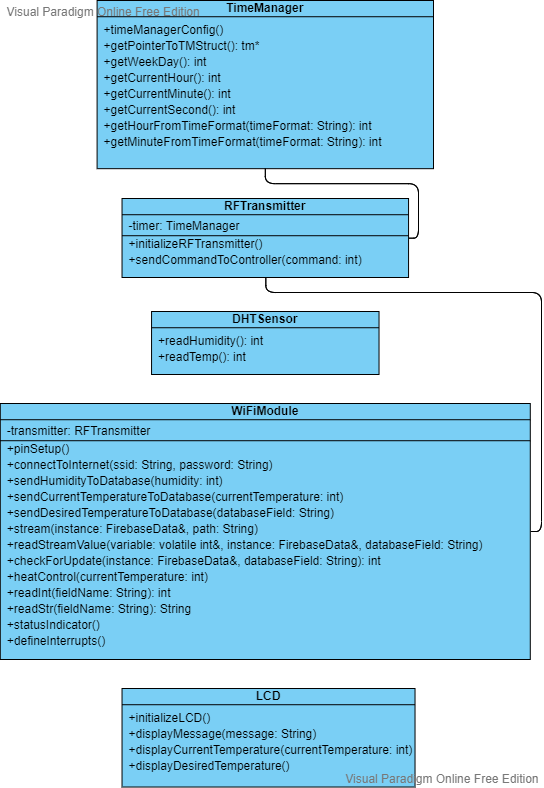
\includegraphics[width=0.6\textwidth]{DiagramaClase.png}
	\caption{Diagramă de clase}
\end{figure}

	Pentru fiecare componentă electronică, ce prezintă funcționalități mai complexe, am creat câte o clasă diferită. Acestea conțin metode ce implementează funcțiile pe care componenta trebuie să le îndeplinească. Cea mai complexă clasă este cea aferentă modulului WiFi, deoarece acesta îndeplinește un rol esențial în cadrul sistemului.

	??compozitie sau agregare??

	Există o relație de compoziție între clasa \textit{WiFiModule} și \textit{RFTransmitter}. În cadrul metodei \textit{heatControl} este necesară o instanță a clasei \textit{RFTransmitter} pentru a putea apela metoda \textit{sendCommandToController}.
 	

\section{Implementarea soluției}

	În acest subcapitol voi prezenta secvențe de cod folosite pentru programarea părții hardware, dar și cod aferent aplicației web.

\subsection{Programare modul ESP8266}

\subsubsection{Inițializări}

	Modulul prezintă o serie vastă de funcționalități și se conectează cu mai multe componente auxiliare. Pentru programarea acestuia am utilizat ArduinoIDE, iar ca și limbaj de programare, C++. 

	Codul este împărțit în trei fișiere cu extensii diferite: .ino, .cpp și .h. În fișierul cu extensia .h se află prototipurile claselor și al metodelor, iar fișierul .cpp conține implementările acestor metode. Fișierul .ino este alcătuit din două funcții: \textit{setup} și \textit{loop}. Prima este utilizată pentru inițializări și se execută o singură dată, la pornirea modulului. În ceea ce privește cea de-a doua funcție, se execută în mod repetitiv până la oprirea alimentării plăcuței WiFi.

\vspace{1em}

	În continuare, voi prezenta funcția \textit{setup} din fișierul .ino și voi explica rolul apelurilor din cadrul acesteia.



\begin{lstlisting}
#include "WiFiModule.h"

WiFiModule wifiModule;
LCD lcd;
TimeManager timeManager;
RFTransmitter rfTransmitter;
DHTSensor dhtSensor;

FirebaseData streamDesiredTemperature;
FirebaseData streamSwitchIntervalsOn;
FirebaseData streamIntervals;


void setup() {
    timeManager.timeManagerConfig();
    lcd.initializeLCD();
    rfTransmitter.initializeRFTransmitter();
    wifiModule.pinSetup();
    wifiModule.connectToInternet("Asus", "vitomir10");
    Firebase.begin(FIREBASE_HOST, FIREBASE_AUTH);
    wifiModule.defineInterrupts();
    wifiModule.stream(streamDesiredTemperature, "/DesiredTempRoom2/Zapier/Value");
    wifiModule.stream(streamSwitchIntervalsOn, "/SwitchIntervalsOn/Value");  
    wifiModule.stream(streamIntervals, "/Intervals");
    delay(500);
}
\end{lstlisting}

\vspace{2em}

	Pentru început, se creează instanțe pentru clasele ale căror funcționalități urmează să fie utilizate, iar în corpul funcției \textit{setup} se vor apela funcții ce țin de inițializare.

	Din clasa \textit{TimeManager} se apelează metoda \textit{timeManagerConfig}, fiind responsabilă de setarea fusului orar. Timpul curent este folosit în modul de funcționare automat, mod în care se ține cont de temperaturile setate de utilizator pe anumite intervale orare. 

	Până se execută toate funcțiile de inițializare, LCD-ul va fi pornit și va afișa mesajul \textit{"Initializing..."}. Pentru ca acest comportament să fie posibil, este necesar apelul metodei \textit{lcd.initializeLCD()}. 	

	Apelarea metodei \textit{initializeRFTransmitter} din cadrul clasei \textit{RFTransmitter} are ca și scop declanșarea procesului de inițializare al transmițătorului. Acesta reprezintă o precondiție pentru transferul de date între modulele senzor și modulul de control.

	Pinii disponibili pe această componentă electronică pot funcționa fie ca intrări, fie ca ieșiri, insă este responsabilitatea programatorului să seteze modul de funcționare a fiecărui pin în parte. Toate aceste configurații le-am grupat în metoda \textit{pinSetup}, al cărei cod îl voi face disponibil.

\vspace{1em}

\begin{lstlisting}
void WiFiModule::pinSetup(){
     pinMode(RELAY_PIN, OUTPUT);
     pinMode(INCREASE_TEMPERATURE_PIN, INPUT);
     pinMode(DECREASE_TEMPERATURE_PIN, INPUT);
     pinMode(LED_BUILTIN, OUTPUT);
}
\end{lstlisting}

\vspace{2em}	

	Pentru identificarea pinilor am definit macrouri, cu nume sugestive, iar cuvintele cheie \textit{INPUT} și \textit{OUTPUT} au fost predefinite în bibliotecile utilizate.

	Majoritatea funcționalităților îndeplinite de acest modul necesită o conexiune validă la internet. Primul pas în acest sens se face prin apelul metodei \textit{connectToInternet}. În cadrul funcției \textit{WiFi.begin()} trebuie menționat numele rețelei la care se conectează și parola. Modulul este programat în așa fel încât timpul alocat conectării la internet să fie de maximum 15 secunde. Dacă acesta este depășit, este posibil să fie o problemă în ceea ce privește conexiunea la internet, iar modulul va funcționa deconectat de la baza de date.
 
	După ce plăcuța WiFi a reușit să se conecteze la internet, următorul pas este identificarea bazei de date. Apelul metodei \textit{Firebase.begin} necesită doi parametri, și anume: adresa bazei de date și cheia secretă. Aceștia sunt utilizați pentru a localiza baza de date, respectiv pentru a oferi acces la aceasta.

	Setarea temperaturii se realizează prin întreruperi. Trebuie definit pinul și frontul semnalului pe care se declanșează întreruperea, dar și numele rutinei de tratare. Toate acestea se realizează în metoda \textit{defineInterrupts}.

	Ultimele apeluri din funcția \textit{setup}, \textit{stream(instance, path)}, au rolul de a seta instanța și câmpul din baza de date pentru care se vor monitoriza schimbările de valoare. Modulul face citiri din baza de date doar când sunt date actualizate, astfel reușind să economisească din resursele disponibile.

\subsubsection{Întreruperile și tratarea acestora}

	În continuare, voi prezenta rutinele de tratare a întreruperilor. Acestea sunt simple, nu consumă multe resurse și, ceea ce este esențial în crearea unor astfel de rutine, execuția lor nu durează mult. De asemenea, utilizez două variabile globale, \textit{increaseDesiredTemperature} și \textit{decreaseDesiredTemperature}, pentru a marca faptul că o procedură de tratare a întreruperii a fost accesată.

\vspace{1em}

\begin{lstlisting}
ICACHE_RAM_ATTR void increaseTemperature() {
    increaseDesiredTemperature = true;
}

ICACHE_RAM_ATTR void decreaseTemperature() {
    decreaseDesiredTemperature = true;
}  
\end{lstlisting}

\vspace{2em}	

	În momentul în care este acționat unul din cele două butoane responsabile cu modificarea temperaturii setate, se declansează execuția unei serii de instrucțiuni. Acestea sunt consumatoare de resurse, motiv pentru care, se execută în interiorul funcției \textit{loop}. 


\vspace{1em}

\begin{lstlisting}
 if(increaseDesiredTemperature || decreaseDesiredTemperature){
    if(increaseDesiredTemperature){
      if(desiredTemperature < MAX_TEMP){
          desiredTemperature++;
          lcd.displayDesiredTemperature();
          if (WiFi.status() == WL_CONNECTED && (!switchIntervalsOn))
          {
              wifiModule.sendDesiredTemperatureToDatabase ("DesiredTempRoom2/Zapier/Value");
          }
      }
      increaseDesiredTemperature = false;
    }else{
        if(desiredTemperature > MIN_TEMP){
          desiredTemperature--;
          lcd.displayDesiredTemperature();
          if (WiFi.status() == WL_CONNECTED && (!switchIntervalsOn))
          {
              wifiModule.sendDesiredTemperatureToDatabase ("DesiredTempRoom2/Zapier/Value");
          }
        }
      decreaseDesiredTemperature = false;
    }
  }
\end{lstlisting}

\vspace{2em}	

	Pentru început, se verifică dacă de la ultima iterație a fost modificată variabila \textit{increaseDesiredTemperature} sau \textit{decreaseDesiredTemperature}. În caz afirmativ, se face o incrementare sau decrementare a valorii temperaturii setate. Pentru ca rezultatul să se afișeze pe LCD cât mai repede, după ajustarea valorii, se face apelul funcției \textit{displayDesiredTemperature}, din cadrul clasei LCD. Astfel, se obține un timp mic de actualizare și o experiență mai bună cu utilizatorul. De asemenea, se examinează modul de funcționare a modulului wireless, conectat, sau nu, la o rețea de internet. In cazul în care există o conexiune validă, valoarea actualizată a temperaturii va fi trimisă în baza de date. O altă condiție necesară este ca modul de funcționare pe intervale orare să fie dezactivat  \textit{!switchIntervalsOn}.

\subsubsection{Mod de operare presetat de utilizator}

	Sistemul este setat asfel încât să ofere posibilitatea utilizatorului de a alege patru intervale orare, cu temperaturi diferite, în timpul zilelor lucrătoare. În ceea ce privește ultimele zile ale săptămânii, sâmbătă și duminică, se pot seta doar două intervale orare pe zi, cu temperaturi diferite.


\vspace{1em}

\begin{lstlisting}
if (WiFi.status() == WL_CONNECTED) {
   wifiModule.sendCurrentTemperatureToDatabase(currentTemperature);
   wifiModule.sendHumidityToDatabase(humidity);
   wifiModule.readStreamValue(switchIntervalsOn, streamSwitchIntervalsOn, "SwitchIntervalsOn/Value");
   if (switchIntervalsOn) {
        int weekDay = timeManager.getWeekDay();
        int currentHour = timeManager.getCurrentHour();
        int currentMinute = timeManager.getCurrentMinute();
        if(wifiModule.checkForUpdate(streamIntervals, "/Intervals") || (!timeIntervalsOperatingMode))
        {
         if (weekDay == 6 || weekDay == 0) {
             String A = wifiModule.readStr("Intervals/Weekend/A");
             String B = wifiModule.readStr("Intervals/Weekend/B");

             int hourA = timeManager.getHourFromTimeFormat(A);
             int minuteA = timeManager.getMinuteFromTimeFormat(A);
             int hourB = timeManager.getHourFromTimeFormat(B);
             int minuteB = timeManager.getMinuteFromTimeFormat(B);

             if ((hourA < currentHour && currentHour < hourB) ||
                 (hourA == currentHour && currentMinute >= minuteA) ||
                 (hourB == currentHour && currentMinute < minuteB)) {
                   wifiModule.readDesiredTemperatureFromDatabase ("Intervals/Weekend/TemperatureAB");
                   endHour = hourB;
                   endMinute = minuteB;
             } else {
                 wifiModule.readDesiredTemperatureFromDatabase ("Intervals/Weekend/TemperatureBA");
                 endHour = hourA;
                 endMinute = minuteA;       
   }
} 
\end{lstlisting}

\vspace{2em}	

	Primele două instrucțiuni au rolul de a încărca în baza de date valoarea temperaturii si a umiditătii. Modul de funcționare a sistemului este salvat într-un câmp al bazei de date, numit \textit{SwitchIntervalsOn/Value}. Acesta este monitorizat prin instalarea unui observator pe câmpul bazei de date. 

	Instrucțiunile ce urmează au rolul de a încadra sistemul în ora, minutul și ziua curentă, iar cu ajutorul acestora, sistemul poate urmări programul de temperaturi setat de către utilizator. Secvența de cod prezentată anterior este utilizată pentru încadrarea zilelor de la sfârșitul săptămânii, sâmbătă si duminică. In cazul în care nu se respectă condițita, se execută secvențele condiționale următoare, împreună cu citirile capetelor intervalelor și valorile temperaturilor corespunzătoare.

\vspace{1em}
	
\begin{lstlisting}
 {
    String A = wifiModule.readStr("Intervals/WorkingDay/A");
    String B = wifiModule.readStr("Intervals/WorkingDay/B");
    String C = wifiModule.readStr("Intervals/WorkingDay/C");
    String D = wifiModule.readStr("Intervals/WorkingDay/D");

    int hourA = timeManager.getHourFromTimeFormat(A);
    int minuteA = timeManager.getMinuteFromTimeFormat(A);
    int hourB = timeManager.getHourFromTimeFormat(B);
    int minuteB = timeManager.getMinuteFromTimeFormat(B);
    int hourC = timeManager.getHourFromTimeFormat(C);
    int minuteC = timeManager.getMinuteFromTimeFormat(C);
    int hourD = timeManager.getHourFromTimeFormat(D);
    int minuteD = timeManager.getMinuteFromTimeFormat(D);


    if ((hourA < currentHour && currentHour < hourB) || (hourA == hourB && currentHour == hourA && currentMinute >= minuteA && currentMinute < minuteB) || (hourA == currentHour && hourB != currentHour && currentMinute >= minuteA) || (hourA != currentHour && hourB == currentHour && currentMinute < minuteB)) {
             wifiModule.readDesiredTemperatureFromDatabase
									("Intervals/WorkingDay/TemperatureAB");
             endHour = hourB;
             endMinute = minuteB;
      } else if ((hourB < currentHour && currentHour < hourC) || (hourB == hourC && currentHour == hourB && currentMinute >= minuteB && currentMinute < minuteC) || (hourB == currentHour && hourC != currentHour && currentMinute >= minuteB) || (hourB != currentHour && hourC == currentHour && currentMinute < minuteC)){
                   wifiModule.readDesiredTemperatureFromDatabase
									("Intervals/WorkingDay/TemperatureBC");
                   endHour = hourC;
                   endMinute = minuteC;
      } else if ((hourC < currentHour && currentHour < hourD) ||  (hourC == hourD && currentHour == hourC && currentMinute >= minuteC && currentMinute < minuteD) || (hourC == currentHour && hourD != currentHour && currentMinute >= minuteC) || (hourC != currentHour && hourD == currentHour && currentMinute < minuteD)) {
                   wifiModule.readDesiredTemperatureFromDatabase
									("Intervals/WorkingDay/TemperatureCD");
                   endHour = hourD;
                   endMinute = minuteD;
     } else {
           wifiModule.readDesiredTemperatureFromDatabase
									("Intervals/WorkingDay/TemperatureDA");
           endHour = hourA;
           endMinute = minuteA;
     }
 }
\end{lstlisting}
\vspace{2em}

\subsubsection{Mod clasic de operare}

	Pe lângă modul automat de funcționare, sistemul este proiectat să poată rula și în mod manual. Acesta presupune menținerea unei temperaturi constante, setate de utilizator, prin butoane, comenzi vocale sau prin intermediul aplicației web. Este important de menționat faptul că acesta consumă mai puține resurse comparativ cu modul de funcționare pe intervale, însă nu oferă același grad de confort. În continuare, voi prezenta o serie de instrucțiuni de cod specifice implementării modului manual.

\vspace{1em}
\begin{lstlisting}
int currentTemperature = dhtSensor.readTemp();
int humidity = dhtSensor.readHumidity();
\end{lstlisting}
\vspace{2em}	

	Prima etapă ce se execută în acest mod este citirea umidității și a temperaturii de la senzorul DHT11. Iar funcțiile responsabile pentru aceste funcționalități sunt apelate la începutul funcției \textit{loop}.

\vspace{1em}
\begin{lstlisting}
wifiModule.heatControl(currentTemperature); 
wifiModule.statusIndicator();
lcd.displayDesiredTemperature();
lcd.displayCurrentTemperature(currentTemperature);
\end{lstlisting}
\vspace{2em}	

	Pentru a face posibilă pornirea/oprirea sistemului de încălzire, este necesar apelul funcției \textit{heatControl}. Acesta trimite comandă atât la electrovalva montată pe calorifer, cât și la centrala termică. De asemenea, este necesar apelul \textit{displayDesiredTemperature} și \textit{displayCurrentTemperature} pentru a afișa temperatura setată și temperatura dorită din cameră. Scopul final este de a permite monitorizarea temperaturii ambientale.

\subsection{Programare plăcuță Arduino}

	Este montată în modulul de control și se conectează la componente auxiliare precum: receptor RF și releu, iar prin intermediul acestora face posibil controlul centralei termice. Codul sursă care face posibil tot acest comportament se află pe plăcuța Arduino. 

\vspace{1em}
	
\begin{lstlisting}
unsigned char dataPackage[3];
uint8_t dataPackageLength = sizeof(dataPackage);
if (driver.recv(dataPackage, &dataPackageLength))
{
    dataPackage[2] = '\0';
    Serial.println((char *) dataPackage);
    int dataPackageInt = atoi((char *) dataPackage);

    if((dataPackageInt/10) == 1){
           commandModule1 = dataPackageInt%10;
           timeFirstModuleSent = millis()/1000;
    }
     else{
            commandModule2 = dataPackageInt%10;
            timeSecondModuleSent = millis()/1000;
        }
        
        Serial.print("Module1:");
        Serial.println(commandModule1);
        Serial.print("Module2:");
        Serial.println(commandModule2);
        if(commandModule1 || commandModule2){
          digitalWrite(7, LOW);
          Serial.println("On");
        }else{
          digitalWrite(7, HIGH);
          Serial.println("Off");
        }
  }
  if((((millis()/1000) - timeFirstModuleSent) >= TIMEOUT && ((millis()/1000) - timeSecondModuleSent) >= TIMEOUT))
  {
          digitalWrite(7, HIGH);
          commandModule1 = 0;
          commandModule2 = 0;
   }
   else if(((millis()/1000) - timeFirstModuleSent) >= TIMEOUT && commandModule2 == 0)
   {
          digitalWrite(7, HIGH);
          commandModule1 = 0;
    }
    else if(((millis()/1000) - timeSecondModuleSent) >= TIMEOUT && commandModule1 == 0) {
          digitalWrite(7, HIGH);
          commandModule2 = 0;
}
\end{lstlisting}
\vspace{2em} 

	Mesajul pe care modulul receptor îl interceptează este format din doi octeți, din care octetul cel mai semnificativ conține numărul de identificare al modulului care a trimis mesajul, iar octetul cel mai puțin semnificativ deține informații legate de natura comenzii. Mesajul recepționat este convertit în întreg datorită faptului că se poate prelucra mai ușor aplicând operații, precum: modulo și div.

	Întotdeauna se salvează momentul în care s-au recepționat informații de la fiecare modul în parte. Este importantă menținerea evidenței, pentru a evita situațiile în care apar întreruperi de transfer prin radio - frecvență. Ca și o măsură de prevenție, dacă modulul de control nu primește comenzi de la modulele senzor un timp mai mare sau egal cu 5 secunde, centrala termică va fi oprită.

	După ce au fost primite comenzi de la ambele module senzor, se execută operație logică de tip SAU, iar în funcție de rezultatul acesteia, va cupla sau decupla releul, ce în continuare controlează centrala termică. Un octet cu valoarea 1 indică pornirea, iar un octet cu valoarea 0 indică oprirea centralei din imobil. De asemenea, ultimele instrucțiuni condiționale din secvența de cod afișată anterior, au rolul de a implementa oprirea de siguranță a sistemului de încălzire. 

	Inițial, se verifică dacă ambele module senzor nu au trimis comenzi de mai mult de 5 secunde. Dacă nu se respectă prima condiție, se examinează cazul în care primul modul are conexiunea întreruptă, iar cel de-al doilea trimite comandă de oprire a sistemului de încălzire. Iar ultima situație care poate apărea este cea în care conexiunea prin radio frecvență la al doilea modul este inactivă de peste 5 secunde, iar primul modul trimite comandă de întrerupere a funcționării centralei. Toate aceste situații apar în cazuri de avarie, iar principala cauză este comunicația precară între modulele senzor și modulul de control. Pentru a preveni defectarea centralei termice, este concepută o măsură de siguranță ce constă în oprirea acesteia.  

\subsection{Realizarea aplicației web}

	Aplicația web face transferul de date cu partea electronică prin intermediul bazei de date \textit{Firebase}. Valorile umidității și a temperaturii se actualizează în aplicația web doar atunci când apar modificări în baza de date. Astfel, se evită citirile repetate și consumatoare de resurse.
	
	În ceea ce privește partea de acces a aplicației, aceasta este găzduită pe un server, la distanță, prin intermediul platformei \textit{Heroku}. Oricine deține adresa aplicației o poate accesa, însă prima pagină care apare la accesare este cea de conectare, iar navigarea poate fi continuată doar în cazul în care utilizatorul deține un cont valid. 
	
\vspace{1em}

\subsubsection{Secvențe de cod esențiale din cadrul implementării aplicației web}

	Pentru a asigura accesul la aplicație doar a persoanelor privilegiate, trebuie creată o pagină de conectare ce să permită verificarea concordanței credențialelor introduse în formular cu cele salvate în baza de date. În cazul unei potriviri, utilizatorul este redirecționat la calea \textit{/home}, aceasta aparținând paginii principale și permite monitorizarea parametrilor ambientali și setarea  temperaturii dorite. Situația în care se introduc credențiale greșite este tratată printr-un mesaj de avertizare, iar utilizatorului i se oferă posibilitatea reintroducerii datelor de conectare.

	Inițial, se preiau informațiile din interfață și se verifică existența utilizatorului cu numele introdus, instrucțiunea ce realizează acest aspect este: \textit{\texttt{user\_to\_login = Users.query.filter\_by(username=username).first()}}. Dacă numele utilizatorului a fost găsit, următorul pas ce trebuie inspectat este potrivirea parolei introduse cu cea salvată în baza de date. Este esențial de luat în considerare faptul că parolele sunt salvate criptate în baza de date, iar înainte de a face comparația cu parola introdusă, este obligatorie și criptarea parolei tastate de utilizator în formularul de conectare. 

	Logica din spatele criptării și verificării ulterioare a parolei o voi prezenta în rândurile ce urmează.

\vspace{3em}	
\begin{lstlisting}	
if user_to_login:
     if bcrypt.check_password_hash(user_to_login.password, password):
           login_user(user_to_login)
           return redirect(url_for('home'))
\end{lstlisting}
\vspace{1em} 	

	Funcția \textit{\texttt{bcrypt.check\_password\_hash}} criptează parola din formular și face si o comparație cu parola din baza de date. În cazul în care corespondența este verificată, utilizatorul devine înregistrat în aplicația web și dobândește drepturi de acces.
  
\vspace{2em}

	Prin intermediul paginii \textit{home} din cadrul aplicației web, utilizatorul are posibilitatea să salveze în baza de date diverse valori ale temperaturilor ce urmează a fi menținute în imobil. În continuare, voi prezenta funcția care se apelează în această situație. Este implementată în \textit{flask} și se execută în momentul în care se ajunge la calea \textit{/home}. 

\vspace{1em}
\begin{lstlisting}
@app.route('/home', methods=['POST', 'GET'])
@login_required
def home():
    status = firebase.get('SwitchIntervalsOn', 'Value')
    if request.method == 'POST':
        variable = request.form.get('outputValue1')
        if variable is not None:
            firebase.put('DesiredTempRoom1/Zapier', 'Value', int(variable))
        else:
            variable = request.form.get('outputValue2')
            firebase.put('DesiredTempRoom2/Zapier', 'Value', int(variable))
    return render_template('controlPage.html', status=status)
\end{lstlisting}
\vspace{2em} 


	 Se utilizează la setarea temperaturii în baza de date, dar și la citirea câmpului \textit{SwitchInvtervalsOn/Value}, ce conține informații referitoare la modul de programare al temperaturilor dorite. 

	Reprezintă o legătură între partea de interfață și logica din spatele aplicației web. Cu alte cuvinte, valoarea introdusă de către utilizator prin intermediul elementelor de intrare din \textit{html}, este transferată în partea responsabilă cu procesarea informațiilor. Prin intermediul funcțiilor puse la dispoziție de un modul implementat în \textit{python}, valorile introduse se transmit mai departe în baza de date.

	Apelul \textit{\texttt{render\_template}} este util pentru a prelucra paginile \textit{html}. Acestea pot conține diverse variabile trimise ca si parametri și pot executa structuri de control, toate acestea pentru a facilita felul în care se construiește interfața cu utilizatorul. Variabila \textit{status} este transmisă mai departe paginii intitulate \textit{controlPage} și este utilizată pentru a seta poziția butonului ce indică modul de funcționare al sistemului.

\vspace{2em}

	În cele ce urmează, voi ilustra modul în care se face o programare a temperaturilor pentru mai multe zile. Voi prezenta traseul pe care informațiile il parcurg, de la introducerea acestora de către utilizator, până la prelucrarea și salvarea lor în baza de date.

	Voi începe prin a expune codul ce face posibilă crearea formularelor utilizate pentru introducerea valorilor temperaturilor și a intervalelor orare. Acestea sunt esențiale pentru interacțiunea între sistem și utilizator.  

\vspace{1em}
\begin{lstlisting}
<div class="form-group">
      <input type="time" class="form-control" name="firstWorkingDayInterval" id="firstWorkingDayInterval" required>
</div>
<div class="form-group">
      <input type="number" class="form-control" name="temperatureFirstWDInterval"
               id="temperatureFirstWDInterval"
               placeholder="Temperature 1" required>
</div>
\end{lstlisting}
\vspace{2em} 

	Primul tip de intrare \textit{html} utilizat este cel pentru formatul timp. Este un câmp predefinit, împărțit în două secțiuni, una pentru alegerea orei, iar cealaltă pentru selectarea minutului.
	
\begin{figure}[H]
   	\centering
    	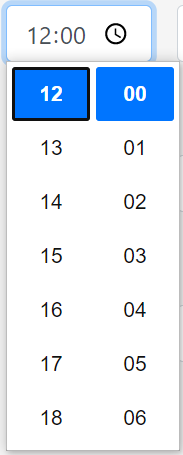
\includegraphics[width=0.4\textwidth]{IntrareDeTipTimp.png}
	\caption{Intrare HTML pentru formatul timp}
\end{figure}

	Cel de-al doilea tip de intrare prezentat, cel de tip numeric, este utilizat pentru setarea valorii temperaturii. Formatul intrarii este creat în așa natură încât să permită un reglaj al valorii, la nivel de unitate.

\begin{figure}[H]
   	\centering
    	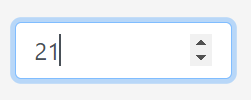
\includegraphics[width=0.3\textwidth]{IntrareDeTipNumeric.png}
	\caption{Intrare HTML pentru formatul numeric}
\end{figure}

	După ce utilizatorul completează toate câmpurile, aceste valori urmează să fie transmise mai departe parții, din cadrul aplicației web, responsabile cu procesarea informațiilor. Transferul datelor se face prin metode de tip \textit{POST}.

	Înainte de salvarea informațiilor în baza de date, este necesară o verificare a acestora. Valorile temperaturilor trebuie să se încadreze în intervalul 15 °C și 32 °C, iar orice depășire a acestor limite nu poate fi stocată. De asemenea, ordinea intervalelor orare trebuie să fie setată într-un mod cronologic. În cazul în care aceste condiții nu sunt respectate, se va afișa un mesaj de eroare adaptat contextului, iar utilizatorului i se oferă posibilitatea reintroducerii datelor.


\vspace{1em}
\begin{lstlisting}
MIN = 15
MAX = 32

timeObjectA = getTime(a)
timeObjectB = getTime(b)
timeObjectC = getTime(c)
timeObjectD = getTime(d)

if int(temperatureAB) < MIN or int(temperatureAB) > MAX or int(temperatureBC) < MIN or int(temperatureBC) > MAX or     			int(temperatureCD) < MIN or int(temperatureCD) > MAX or int(temperatureDA) < MIN or int(temperatureDA) > MAX:
            flash('The values of temperatures should be between 15 and 32 degrees!', 'warning')
else:
	if timeObjectA < timeObjectB < timeObjectC < timeObjectD:
      		try:
              	firebase.put('Intervals/WorkingDay', 'A', a)
              	firebase.put('Intervals/WorkingDay', 'B', b)
              	firebase.put('Intervals/WorkingDay', 'C', c)
              	firebase.put('Intervals/WorkingDay', 'D', d)

              	firebase.put('Intervals/WorkingDay', 'TemperatureAB', int(temperatureAB))
              	firebase.put('Intervals/WorkingDay', 'TemperatureBC', int(temperatureBC))
              	firebase.put('Intervals/WorkingDay', 'TemperatureCD', int(temperatureCD))
              	firebase.put('Intervals/WorkingDay', 'TemperatureDA', int(temperatureDA))
       	except Exception as err:
                	flash('An error ocurred while setting intervals: {0}'.format(err), 'warning')
	else:
		flash('Time intervals must be set chronologically!', 'warning')
return render_template('schedulingPage.html')
\end{lstlisting}
\vspace{2em} 

	Prima instrucțiune condițională utilizată în codul prezentat anterior, are rolul de a determina dacă valorile temperaturilor introduse se încadrează în intervalul acceptat de sistem și de aplicația web.  

	Pe de altă parte, pentru a putea stabili dacă există o ordine cronologică, se apelează funcția \textit{getTime} cu datele pe care le citim de la intrarea pentru formatul de tip timp. Se creează obiecte ce conțin data, ora și minutul curent pentru fiecare interval în parte. Datorită faptului că aceste obiecte sunt predefinite in \textit{python}, se pot aplica operații de comparație asupra lor. 

	Implementarea funcției de încapsulare a valorilor intervalelor o voi prezenta în rândurile ce urmează, împreună cu explicațiile de cod aferente. 

\vspace{1em}
\begin{lstlisting}
def getTime(timeFormat):
    hour = getHourFromTimeFormat(timeFormat)
    minute = getMinuteFromTimeFormat(timeFormat)

    now = datetime.now(pytz.timezone('Europe/Bucharest'))
    dateTimeObject = datetime(now.year, now.month, now.day, hour, minute)

    return dateTimeObject
\end{lstlisting}
\vspace{2em} 

	Apelul \textit{getHourFromTimeFormat} și \textit{getMinuteFromTimeFormat} sunt utilizate pentru a despărți șirul de caractere ce conține ora și minutul setat de către utilizator. Obiectele predefinite în \textit{python} pentru stocarea datei și timpului prezintă ca și câmpuri obligatorii: anul, luna, ziua, ora și minutul. Ca și intrare de la utilizator primim doar ora și minutul, iar pentru crearea obiectului, restul valorilor ne sunt puse la dispoziție prin intermediul unui modul \textit{python}, ce are setat fusul orar actual. În urma apelului funcției \textit{datetime} sunt returnate obiecte ce conțin data curentă, ora și minutul capetelor intervalelor introduse de utilizator. Pe aceste obiecte se vor executa operații de comparație pentru a determina dacă ordinea este una cronologică.

	Intr-un final, după ce datele au fost validate, urmează salvarea acestora în baza de date. Pentru a implementa acest aspect, se utilizează suita de apeluri \textit{firebase.put}, care primesc ca și parametrii: numele câmpului unde urmează să se facă stocarea, împreună cu informațiile aferente.


\begin{figure}[H]
   	\centering
    	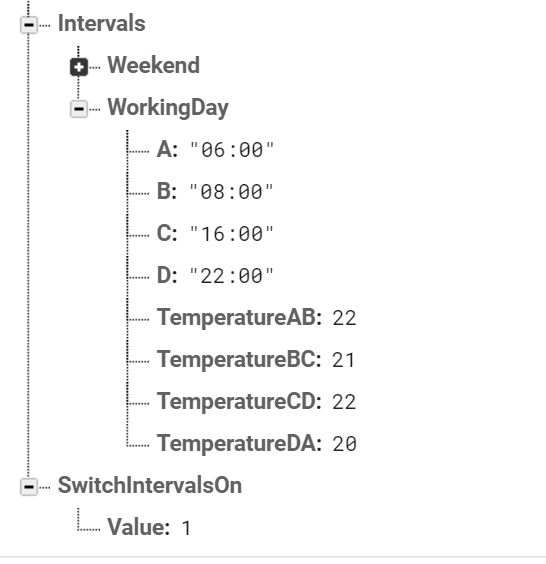
\includegraphics[width=0.8\textwidth]{IntervalsWorkingDays.png}
	\caption{Stocare program intervale orare}
\end{figure}

\subsection{Probleme întâmpinate în timpul realizării proiectului}

\subsubsection{Forța contraelectromotoare a bobinei}

	Electrovalvele sunt formate dintr-un solenoid. Aplicarea tensiunii la bornele acestuia duce la generarea unui câmp electromagnetic, care la rândul său acționează un obturator. Astfel, se realizează închiderea/deschiderea circuitului de apă. Este important de menționat faptul că solenoidul înmagazinează curent, iar întreruperea alimentarii electrice a acestuia produce o descărcare, ce se manifestă prin apariția unor fluctuații de tensiune în circuit. Prezența acestor fluctuații poate duce la arderea celorlalte componente electronice, dar și la o uzură accentuată a releelor de comandă. De asemenea, descărcarea solenoidului produce apariția unor scântei între contactele releului, determinând perturbații în intreg sistemul. Un exemplu de disfuncționalitate cu care m-am confruntat din aceasă cauză, a fost dereglarea temperaturii setate, în momentul în care modulul ESP8266 trimitea comandă de inchidere a elevtrovalvei.   

\subsubsection{Vibrațiile contactelor metalice ale întrerupătoarelor}

	Pentru a putea modifica valoarea temperaturii setate a fi menținute în imobil, se utilizează butoane fizice, legate prin conductori eletrici la modulele WiFi. Din punct de vedere funcțional, acestea pot avea comportament neașteptat, cauzat de vibrațiile fine care se produc între contactele metalice ale întrerupătorului. Frecvența cu care microcontrolerul citește semnalul provenit de la buton este suficient de mare, astfel încât, să poată sesiza inclusiv o vibrație ca fiind o apăsare distinctă. Prin urmare, se întâmpla ocazional ca intenția utilizatorului de a incrementa sau decrementa cu o unitate temperatura setată, să se traducă în modificarea acesteia cu mai multe unități. Soluția pe care am implementat-o în această situație, a fost realizarea și montarea unor filtre trece jos pentru fiecare buton în parte. Rolul acestora este de a permite trecerea doar a semnalelor cu frecvențe mici, iar cele de frecvențe mari, perturbațiile, fiind oprite. Capturile de ecran din cadrul capitolului 3, prezintă semnalul înainte de filtrare \ref{fig:InainteDeFiltru}, dar și după aceasta \ref{fig:DupaFiltru}.

\subsubsection{Amorsarea instalației cu apă}

	Pompa de apă pe care am utilizat-o în circuit, nu prezintă funcționalitate de autoamorsare. Prin urmare, prima tentativă de umplere a circuitului cu apă, a constat în desfacerea unei îmbinări a circuitului și introducerea apei cu o seringă prin aceasta. Din cauza faptului că instalația prezintă multe coturi, iar introducerea apei nu o faceam din punctul cel mai înalt, procentajul de umplere al circuitului nu era satisfăcător. Ca și disfuncționalitate, se manifesta prin faptul că pompa de apă de dezamorsa în timpul funcționării. Într-un final, am decis să montez un aerisitor în punctul cel mai înalt al instalației, iar introducerea apei să se facă prin acesta. Astfel, volumul de aer din circuit a fost redus considerabil, ducând la eliminarea situațiilor de dezamorsare a pompei.

\subsubsection{Conflict de date apărut la transferul prin radio - frecvență}

	Ambele transmițătoare utilizate în cadrul machetei funcționează la aceeași frecvență, 433 Mhz. Transferul datelor se face către un singur receptor, montat pe modulul de comandă al centralei termice. Din punct de vedere funcțional, apăreau probleme în momentul în care ambele transmițătoare făceau transfer simultan. Datele nu mai ajungeau să fie recepționate de către receptor, ajungând la pierderea comenzilor. Modulele wireless sunt conectate la un server prin intermediul căruia citesc data și ora curentă. Utilizând acest aspect, am programat modulele astfel încât să facă transferul de date concurent. Un modul va transfera la secundă pară, pe când celălalt la secundă impară. 

\section{Testarea soluției}

	În orice proces ce implică dezvoltare de proiecte de o complexitate mai mare, etapa de testare este una esențială. Aceasta presupune identificarea erorilor sistemului, înainte de a fi pus în producție. Cazurile de test trebuie proiectate astfel încât să cuprindă toate situațiile care pot produce abateri de la comportamentul standard. 

	În ceea ce privește proiectul prezentat, testarea a vizat două mari componente: aplicația web și instalația pentru circuitul de apă. \textit{Flask} oferă posibilitatea de creare de teste unitare pentru proiectele realizate prin intermediul lui. Pe lângă aceasta, permite și analiza procentului de acoperire al întregii aplicații prin testele scrise.

	Voi începe prin a prezenta partea de validare a aplicației web. Am realizat o suită de 50 de teste, pe care am împărțit-o în 3 mari categorii. Prima categorie conține cazurile de test comune pentru toți utilizatorii, funcționalități care sunt valabile indiferent de rolul persoanei autentificate aplicației. Am încercat să abordez o manieră exhaustivă, prin simularea tuturor situațiilor de eroare, dar și de reușită. Printre cazurile mai importante de test care se încadrează în această categorie sunt:

	\begin{itemize}
			\setlength{\itemindent}{2em}
			\itemsep0em
			\item Verificarea faptului că pentru a putea realiza orice funcționalitate din aplicația web, trebuie să existe un utilizator conectat. Altfel, accesul este obligatoriu să fie interzis.
			\item Încercarea de conectare utilizând un cont inexistent, trebuie interzisă și avertizată printr-un mesaj de eroare.
			\item Verificarea funcției de criptare a parolei utilizatorului.
			\item Verificarea posibilității de conectare la aplicația web.
			\item Introducerea parolei greșite în momentul conectării.
			\item Testarea funcționalității de deconectare.
			\item Acitvare/Dezactivare mod de lucru cu intervale orare
			\item Controlul posibilității de setare a intervalelor pentru zile lucrătoare, dar si pentru cele de la sfârșitul săptămânii. De asemenea, cazurile acestea de test se împart în mai multe. Situația în care acestea nu sunt setate în ordine cronologică și situația în care vreo valoare a temperaturii nu se încadrează în intervalul 15 °C - 32 °C.
			\item Funcția de schimbare a parolei, implică verificarea situațiilor în care: parola curentă nu este validă, parolele introduse nu se potrivesc, noua parolă este prea scurtă, noua parolă nu conține majusculă și situația în care noua parolă nu conține cifră.
			\item Verificarea funcției de setare a temperaturii pentru ambele camere.
	\end{itemize} 

\vspace{2em}

	Cea de-a doua categorie este dedicată testelor unitare pentru utilizatorii care nu au drepturi de administrator. În principiu, aici se verifică faptul că doar aministratorii au acces la funcționalitățile privilegiate. Sunt validate cazurile de test precum:
 
	\begin{itemize}
			\setlength{\itemindent}{2em}
			\itemsep0em
			\item Un cont fără drept de aministrator nu este autorizat pentru crearea de alte conturi.
			\item Nu este permis accesul pentru a vedea lista de conturi, a șterge un cont, a oferi drepturi de administrator sau a șterge drepturi de aministrator.
	\end{itemize} 

\vspace{2em}

	În cele din urmă, ultima categorie cuprinde testarea doar a funcționalităților dedicate administratorilor. Se verifică:

	\begin{itemize}
			\setlength{\itemindent}{2em}
			\itemsep0em
			\item Posibilitatea de creare de conturi noi.
			\item Interzicerea accesului de a crea un cont nou dacă: parolele nu se potrivesc, parola introdusă este prea scurtă, nu conține majusculă sau nu conține cel puțin o cifră.
			\item Ștergerea unui cont.
			\item Incercarea de ștergere a unui cont inexistent.
			\item Acordarea drepturilor de administrator unui anumit cont.
			\item Acordarea drepturilor de administrator unui cont inexistent.
			\item Retragerea drepturilor de administrator.
			\item Retragerea drepturilor de administrator pentru un cont inexistent.
	\end{itemize} 

	Este important ca prin testele create să acoperim un procent cât mai mare din întreaga aplicație. Cu toate acestea, trebuie menționat faptul că, procentul de acoperire nu este un indicator al calității testelor, ci doar reprezintă cât de multe funcționalități sunt acoperite prin cazurile de test.

\begin{figure}[H]
	\centering
    	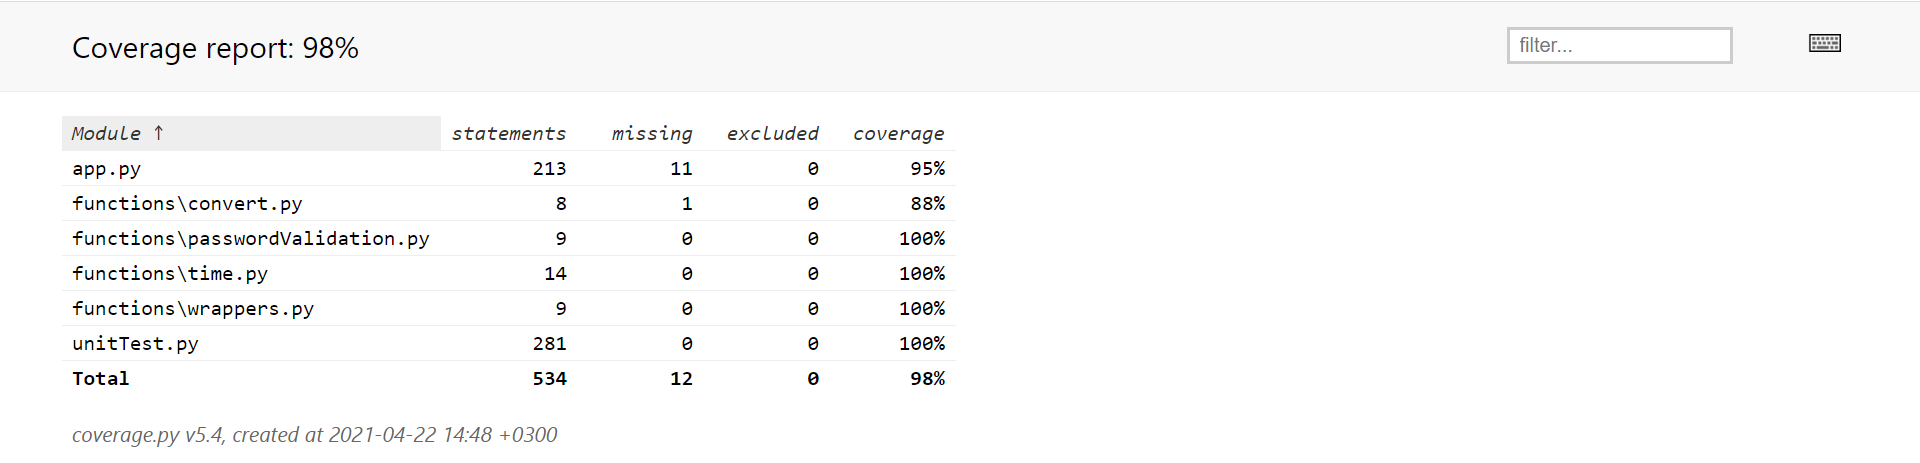
\includegraphics[width=1\textwidth, height=4.5cm]{CoverageReport.png}
	\caption{Procent de acoperire}
\end{figure}    

\vspace{2em}

	Partea de verificare a instalației de apă a fost una mai simplă. După finalizarea lipiturilor conductelor de cupru și montarea garniturilor la fiecare îmbinare, a fost necesară o verificare a faptului că etanșeitatea este asigurată. Procesul a constat în introducerea unei presiuni de 2 bari, pe care am menținut-o în circuit un timp de 10 minute. În toată această perioadă, am monitorizat, cu ajutorul manometrului pompei de aer, faptul că presiunea rămâne constantă. Pentru a mă asigura că pompa de apă și electrovalvele funcționează corespunzător, am folosit o sursă de tensiune de 12 volți și am alimentat fiecare componentă electrică în parte. 


	

\listoffigures

\listoftables
\bibliographystyle{unsrt}
\bibliography{bibfile.bib}

\end{document}